\documentclass[12pt]{article}

\usepackage{makeidx}

\usepackage{graphicx, color}
\usepackage{tikz}
\DeclareGraphicsRule{*}{mps}{*}{}
\usepackage{linalgjh}
\usepackage{hyperref}
\usepackage[toc]{glossaries}

%Change the next line as appropriate for your course.
\newcommand{\webworkurl}{http://webwork.math.ucdavis.edu/webwork2/COURSETITLE/}

\def\nn{\nonumber}

\newtheorem{theorem}{Theorem}[section]
\newtheorem{lemma}[theorem]{Lemma}
\newtheorem{proposition}[theorem]{Proposition}
\newtheorem{corollary}[theorem]{Corollary}


\newenvironment{definition}[1][Definition]{\begin{trivlist}
\item[\hskip \labelsep {\bfseries #1}]}{\end{trivlist}}
\newenvironment{example}[1][Example]{\begin{trivlist}
\item[\hskip \labelsep {\bfseries #1}]}{\end{trivlist}}
\newenvironment{remark}[1][Remark]{\begin{trivlist}
\item[\hskip \labelsep {\bfseries #1}]}{\end{trivlist}}

\DeclareMathOperator{\tr}{tr}
\DeclareMathOperator{\rref}{RREF}

% sideremark
\def\sideremark#1{\ifvmode\leavevmode\fi\vadjust{\vbox to0pt{\vss
\hbox to 0pt{\hskip\hsize\hskip1em
\vbox{\hsize3cm\tiny\raggedright\pretolerance10000
 \noindent #1\hfill}\hss}\vbox to8pt{\vfil}\vss}}}


\newcommand{\edz}[1]{\sideremark{#1}}
\def\idx#1{{\em #1\/}} % ****

\newcommand{\1}{{\rm 1\hspace*{-0.4ex}%
\rule{0.1ex}{1.52ex}\hspace*{0.2ex}}}

\DeclareMathOperator{\cofactor}{cofactor}
\DeclareMathOperator{\spa}{span}
\DeclareMathOperator{\nul}{null}


\makeindex

\makeglossaries

\begin{document}

\title{Linear Algebra in Twenty Five Lectures}

\author{Tom Denton and Andrew Waldron}


\maketitle

\begin{center}
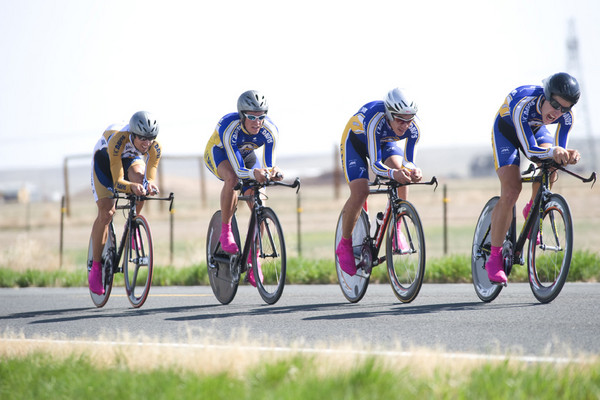
\includegraphics[scale=.6]{bikes.jpg}\\[8mm]
 {Edited by Rohit Thomas}
\end{center}

\newpage

\tableofcontents


\newpage



\section*{Preface}

This ``book'' grew out of a series of twenty five lecture notes for a sophomore linear algebra class
taught at the University of California, Davis. The audience was primarily engineering students and
students of pure sciences, some of whom may go on to major in mathematics.
It was motivated by the lack of a book that 
 taught students basic structures of linear algebra without overdoing mathematical rigor
 or becoming a mindless exercise in crunching recipes at the cost of fundamental understanding.
In particular we wanted a book that was suitable for all students, not just math majors, that focussed
on concepts and developing the ability to think in terms of abstract structures in order to address the 
dizzying array of seemingly disparate applications that can all actually be addressed with linear algebra methods.

In addition we had practical concerns. We wanted to offer students a online version of the book for free, both because
we felt it our academic duty to do so, but also because we could seamlessly link an online book to a myriad of other 
resources--in particular WeBWorK exercises and videos. We also wanted to make the LaTeX source available to other instructors
so they could easily customize the material to fit their own needs. Finally, we wanted to restructure the way the course 
was taught, by getting the students to direct most of their effort at more difficult problems where they had to think through
concepts,  present well-thought out logical arguments and learn to turn word problems into ones where the usual array of linear algebra recipes could take over.

\subsection*{How to Use the Book}

At the end of each chapter there is a set of review questions. Our students found these very difficult, mostly because they 
did not know where to begin, rather than needing a clever trick. We designed them this way to ensure that students grappled with 
basic concepts. Our main aim was for students to master these problems, so that we could ask similar high caliber problems on midterm and
final examinations. This meant that we did have to direct resources to grading some of these problems. For this we used two tricks.
First we asked students to hand in more problems than we could grade, and then secretly selected a subset for grading.
Second, because there are more review questions than what an individual student could handle, we split the class into groups of three
or four and assigned the remaining problems to them for grading. Teamwork is a skill our students will need in the workplace;
also it really enhanced their enjoyment of mathematics.

Learning math is like learning to play a violin--many ``technical exercises'' are
necessary before you can really make music! Therefore, each chapter has a set of dedicated WeBWorK ``skills problems'' where students can test that they have mastered basic linear algebra skills. The beauty of WeBWorK is that students get instant feedback and
problems can be randomized, which means that although students are working on the same types of problem, they cannot simply 
tell each other the answer. Instead, we encourage them to explain to one another how to do the WeBWorK exercises. 
Our experience is that this way, students can mostly figure out how to do the WeBWorK problems among themselves, freeing up discussion groups and office hours for weightier issues.  Finally, we really wanted our students to carefully read the book. Therefore, each chapter has several very simple WeBWorK ``reading problems''. These appear as links at strategic places. They are very simple problems that can 
answered rapidly if a student has read the preceding text.

\subsection*{The Material}

We believe the entire book can be taught in twenty five fifty minute lectures to a sophomore audience that has been exposed to a one year 
calculus course. Vector calculus is useful, but not necessary preparation for this book, which attempts to be self-contained.
Key concepts are presented multiple times, throughout the book, often first in a more intuitive setting, and then again 
in a definition, theorem, proof style later on. We do not aim for students to become agile mathematical proof writers, but we 
do expect them to be able to show and explain why key results hold. We also often use the review exercises to let students discover
key results for themselves; before they are presented again in detail later in the book. 

Linear algebra courses run the risk of becoming a conglomeration of learn-by-rote recipes involving arrays filled with numbers.
In the modern computer era, understanding these recipes, why they work, and what they are for is more important than ever.
Therefore, we believe it is crucial to change the students' approach to mathematics right from the beginning of the course. Instead of
them asking us ``what do I do here?'', we want them to ask ``why would I do that?'' This means that students need to start to think in terms of
abstract structures. In particular, they need to rapidly become conversant in sets and functions--the first WeBWorK set will help 
them brush up these~skills.

There is no best order to teach a linear algebra course. The book has been written such that instructors can reorder the chapters (using the LaTeX source) in any (reasonable) order and still have a consistent text. We hammer the notions of abstract vectors and linear transformations hard and  early, while at the same time giving students the basic matrix skills necessary to perform computations.
Gaussian elimination is followed directly by an ``exploration chapter'' on the simplex algorithm to open students minds to problems 
beyond standard linear systems ones. Vectors in ${\mathbb R}^n$ and general vector spaces are presented back to back so that students
are not stranded with the idea that vectors are just ordered lists of numbers. To this end, we also labor the notion of all functions from a set to 
the real numbers. In the same vein linear transformations and matrices are presented hand in hand. Once students see that a linear map
is specified by its action on a limited set of inputs, they can already understand what a basis is.
All the while students are studying linear systems and their solution sets, so after determinants are introduced right after  matrices.
This material can proceed rapidly since elementary matrices were already introduced with Gaussian elimination. Only then is a careful 
discussion of spans, linear independence and dimension given to ready students for a thorough treatment of eigenvectors and
diagonalization. The dimension formula therefore appears quite late, since we prefer not to elevate rote computations of column and
row spaces to a pedestal. The book ends with applications--least squares and singular values. These are a fun way to end any lecture course.
It would also be quite easy to spend any extra time on systems of differential equations and simple Fourier transform problems.

\newpage 
\noindent
One possible distribution of twenty five fifty minute lectures might be:
\begin{center}
\begin{tabular}{lr}
Chapter & Lectures\\ \hline
What is Linear Algebra?&1\\
Systems of Linear Equations&3\\
The Simplex Method&1\\
Vectors in Space, $n$-Vectors&1\\
Vector Spaces&1\\
Linear Transformations&1\\
Matrices&3\\
Determinants&2\\
Subspaces and Spanning Sets&1\\
Linear Independence&1\\
Basis and Dimension&1\\
Eigenvalues and Eigenvectors&2\\
Diagonalization&1\\
Orthonormal Bases and Complements&2\\
Diagonalizing Symmetric Matrices&1\\
Kernel, Range, Nullity, Rank&1\\ 
Least Squares and Singular Values&1\\ \hline\end{tabular}
\end{center}

Creating this book has taken the labor of many people. Special  thanks are due to Katrina Glaeser  and Travis Scrimshaw
for shooting many of the videos and LaTeXing their scripts. Rohit Thomas wrote many of the WeBWorK problems. Bruno 
Nachtergaele and Anne Schilling provided inspiration for creating a free resource for all students of linear algebra.
Dan Comins helped with technical aspects. A University of California online pilot grant helped fund the graduate students
who worked on the project. Most of all we thank our students who found many errors in the book and taught us how to teach this material!

Finally, we admit the book's many shortcomings: clumsy writing, low quality artwork and low-tech video material. We welcome
anybody who wishes to contribute new material---WeBWorK problems, videos, pictures---to make this resource a better one and are glad to hear of any typographical errors,
mathematical fallacies, or simply ideas how to improve the book.

\vspace{1cm}

\noindent
David, Tom, and Andrew


%These linear algebra lecture notes are designed to be presented as twenty five, fifty minute lectures
%suitable for sophomores likely to use the material for applications but still requiring
%a solid foundation in this fundamental branch of mathematics. The main idea of the course is
%to emphasize the concepts of vector spaces and linear transformations as mathematical
%structures that can be used to model the world around us. Once ``persuaded'' of this truth, students
%learn explicit skills such as Gaussian elimination and diagonalization in order that vectors and linear transformations
%become calculational tools, rather than abstract mathematics.
%
%In practical terms, the course aims to produce students who can perform computations with large linear systems
%while at the same time understand the concepts behind these techniques. Often-times when a problem can be
%reduced to one of linear algebra it is ``solved''. These notes 
%do not devote much space to applications (there are already a plethora of textbooks with titles involving some
%permutation of the words ``linear'', ``algebra'' and ``applications''). Instead, they attempt to explain the fundamental
%concepts carefully enough that students will realize for their own selves when the particular application they encounter
%in future studies is ripe for a solution via linear algebra.
%
%There are relatively few worked examples or illustrations in these notes, this material is instead covered by a series
%of ``linear algebra how-to videos''. They can be viewed by clicking on the take one icon~\raisebox{-.2cm}{
\includegraphics[scale=.05]{take1.jpg}}.
%The \hyperlink{scripts}{``scripts''} for these movies are found at the end of the notes if students prefer to read this material in a traditional format
%and can be easily reached via the script icon~\raisebox{-.2cm}{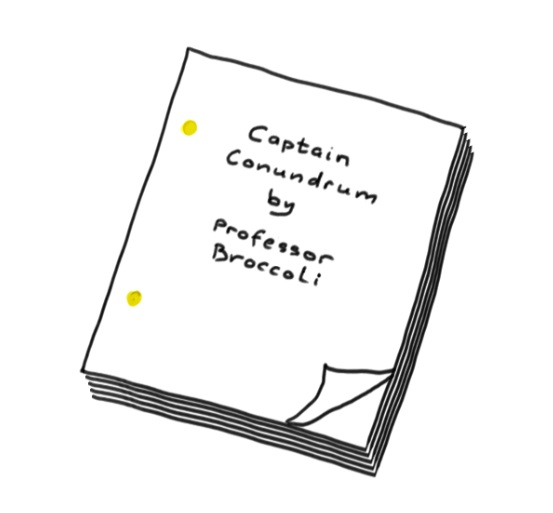
\includegraphics[scale=.05]{script.jpg}}. Watch an introductory video below:
%
%\videoscriptlink{intro.mp4}{Introductory Video}{intro}
%
%The notes are designed to be used in conjunction with a set of online homework exercises which help the students read the
%lecture notes and learn 
%basic linear algebra skills. Interspersed among the lecture notes are links to simple online problems that
%test whether students are actively reading the notes. In addition there are two sets of sample midterm problems with solutions as well
%as a sample final exam. 
%There are also a set of ten online assignments which are usually collected weekly.
%The first assignment is designed to ensure familiarity with some basic mathematic notions (sets, functions, logical quantifiers and basic methods of proof). The remaining nine assignments are devoted to the usual matrix and vector gymnastics expected from 
%any sophomore linear algebra class. These exercises are all available at
%
%\begin{quote}
%\href{\webworkurl}{\webworkurl}
%\end{quote}
%
%\noindent
%Webwork is an open source, online homework system which originated at the University of Rochester. It can efficiently check whether a student
%has answered an explicit, typically computation-based, problem correctly. The problem sets chosen to accompany these
%notes could contribute roughly  20\% of a student's grade, and ensure that basic computational skills are mastered.
%Most students rapidly realize that it is best to print out the Webwork assignments and solve them on paper before 
%entering the answers online. Those who do not tend to fare poorly on midterm examinations. We have found that there 
%tend to be relatively few questions from students in office hours about the Webwork assignments. Instead, by assigning 20\%
%of the grade to written assignments drawn from  problems chosen randomly from the review exercises at the end of each lecture, the
%student's focus was primarily on understanding ideas. They range from simple tests of understanding of the material in the lectures
%to more difficult problems, all of them require thinking, rather than blind application of mathematical ``recipes''. 
%Office hour questions reflected this and offered an excellent chance
%to give students tips how to present written answers in a way that would convince the person grading their work that they deserved full credit!
%
%Each lecture concludes with references to the comprehensive online textbooks of Jim Hefferon and Rob Beezer:
%
%\begin{quote}
%\href{http://joshua.smcvt.edu/linearalgebra/}{http://joshua.smcvt.edu/linearalgebra/}\\[5mm]
%\href{http://linear.ups.edu/index.html}{http://linear.ups.edu/index.html}
%\end{quote}
%and the notes are also hyperlinked to Wikipedia where students can rapidly access further details and background material
%for many of the concepts. Videos of linear algebra lectures are available online from at least two sources:
%\begin{itemize}
%\item The Khan Academy, \\ \href{http://www.khanacademy.org/?video#Linear Algebra}{http://www.khanacademy.org/?video\#Linear Algebra}
%\item MIT OpenCourseWare, Professor Gilbert Strang, \\ \href{http://ocw.mit.edu/courses/mathematics/18-06-linear-algebra-spring-2010/video-lectures/}{http://ocw.mit.edu/courses/mathematics/18-06-linear-algebra-spring\\ -2010/video-lectures/}
%\end{itemize}
%There are also an array of useful commercially available texts. A non-exhaustive list includes
%\begin{itemize}
%\item ``Introductory Linear Algebra, An Applied First Course'', B. Kolman and D. Hill, Pearson 2001.
%\item ``Linear Algebra and Its Applications'', David C. Lay, Addison--Weseley 2011.
%\item ``Introduction to Linear Algebra'', Gilbert Strang, Wellesley Cambridge Press 2009.
%\item ``Linear Algebra Done Right'', S. Axler, Springer 1997.
%\item ``Algebra and Geometry'', D. Holten and J. Lloyd, CBRC, 1978.
%\item ``Schaum's Outline of Linear Algebra'', S. Lipschutz and M. Lipson, McGraw-Hill 2008.
%\end{itemize}
%A good strategy is to find your favorite among these in the University Library.
%
%There are many, many useful online math resources. A partial list is given in Appendix~\ref{othersources}.
%
%Students have also started contributing to these notes. Click \hyperlink{student_creations}{here} to see some of their work.
%
%There are many ``cartoon'' type images for the important theorems and formal\ae\ . In a classroom with a projector, a useful technique for instructors
%is to project these using a computer. They provide a colorful relief for  students from (often illegible) scribbles on a blackboard.
%These can be downloaded at:
%
%\begin{center}
%\href{http://math.ucdavis.edu/~linear/lecture_materials}{Lecture Materials}
%\end{center}
%
%There are still many errors in the notes, as well as awkwardly explained concepts. An army of 400 students, Fu Liu, Stephen Pon and Gerry Puckett have already found
%many of them. Rohit Thomas has spent a great deal of time editing these notes and the accompanying webworks and has improved them immeasurably. 
%Katrina Glaeser and Travis Scrimshaw have spent many hours shooting and scripting the how-to videos and taken these notes to a whole new level!
%Anne Schilling shot a great guest video.
%We also thank Captain Conundrum\index{Captain Conundrum} for providing us his solutions to the sample
%midterm and final questions. The review exercises would provide a better survey of what linear algebra really is if there were more ``applied''
%questions.  We welcome your contributions!
%
%\begin{quote}
%Andrew and Tom.
%\end{quote}

 
\newpage




\input{notes1}

\input{notes2}

\input{notes3}

\input{notes4}

\input{notes5}

\input{notes6}

\input{notes7}

\input{notes8}

\input{notes9}

\input{notes10}


\input{notes11}

\input{notes12}

\input{notes13}

\input{notes14}

\input{notes15}

\input{notes16}

\input{notes17}

\input{notes18}

\input{notes19}



\input{notes20}

\input{notes21}

\input{notes22}

\input{notes23}

\input{notes24}

\input{notes25}

\appendix

\chapter{Sample First Midterm}

Here are some worked problems typical for what you might expect on a first midterm examination.
\label{sample1}

\begin{enumerate}
\item Solve the following linear system.  Write the solution set in vector form.  Check your solution.  Write one particular solution and one homogeneous solution, if they exist.  What does the solution set look like geometrically?
$$
\begin{array}{rrrrrr}
x &+&3y & &&= 4\\[1mm]
x &-& 2y &+& z &= 1\\[1mm]
2x &+&y &+& z &= 5\\[1mm]
\end{array}
$$

\item
Consider the system of equations
$$
\left\{
\begin{array}{rrrrrrrrr}
x&&&-&z&+&2w&=&-1\\[2mm]
x&+&y&+&z&-&w&=&2\\[2mm]
&-&y&-&2z&+&3w&=&-3\\[2mm]
5x&+&2y&-&z&+&4w&=&1\\[2mm]
\end{array}
\right. 
$$
\begin{enumerate}
\item Write an augmented matrix for this system.
\item Use elementary row operations to find its reduced row echelon form.
\item Write the solution set for the system in the form $$S=\{X_0+\sum_i \mu_i Y_i:\mu_i\in \mathbb R\} .$$
\item What are the vectors $X_0$ and $Y_i$ called {\it and} which matrix equations do they solve?
\item Check separately that $X_0$ and each $Y_i$ solve the matrix systems you claimed they solved in part (d).
\end{enumerate}

\item Use row operations to invert the matrix
$$
\begin{pmatrix}
1&2&3&4\\
2&4&7&11\\
3&7&14&25\\
4&11&25&50
\end{pmatrix}
$$

\item Let $M = \left ( \begin{array}{cc} 2 & 1 \\ 3 & -1 \end{array}  \right )$.  Calculate $M^TM^{-1}$.  Is $M$ symmetric?  What is the trace of the transpose of $f(M)$, where $f(x) = x^2 -1$?

\item In this problem $M$ is the matrix
$$
M=\begin{pmatrix}\cos\theta & \sin\theta \\ -\sin\theta&\cos\theta\end{pmatrix}
$$
and $X$ is the vector
$$
X=\begin{pmatrix}x\\y \end{pmatrix}\, .
$$
Calculate all possible dot products between the vectors $X$ and $MX$. Compute the lengths of $X$ and $MX$.
What is the angle between the vectors $MX$ and $X$. Draw a picture of these vectors in the plane. For what values
of $\theta$ do you expect equality in the triangle and Cauchy--Schwartz inequalities?

\item Let $M$ be the matrix
$$
\begin{pmatrix}
1&0&0&1&0&0\\
0&1&0&0&1&0\\
0&0&1&0&0&1\\
0&0&0&1&0&0\\
0&0&0&0&1&0\\
0&0&0&0&0&1
\end{pmatrix}
$$
Find a formula for $M^k$ for any positive integer power~$k$. Try some simple examples like $k=2,3$ if confused.



\item What does it mean for a function to be linear?  Check that integration is a linear function from $V$ to $V$, where $V = \{ f: \mathbb{R} \to \mathbb{R} \mid f \textrm{ is integrable}\}$ is a vector space over $\mathbb{R}$ with usual addition and scalar multiplication.


\item What are the four main things we need to define for a vector space?  Which of the following is a vector space over $\mathbb{R}$?  For those that are not vector spaces, modify one part of the definition to make it into a vector space.
\begin{enumerate}
\item $V = \{ \textrm{ $2 \times 2$ matrices with entries in $\mathbb{R}$} \}$, usual matrix addition, and $k \cdot \left ( \begin{array}{cc} a & b \\ c & d \end{array}  \right ) = \left ( \begin{array}{cc} ka & b \\ kc & d \end{array}  \right )$ for $k \in \mathbb{R}$.

\item $V = \{ \textrm{polynomials with complex coefficients of degree $\leq 3$} \}$, with usual addition and scalar multiplication of polynomials.

\item $V = \{ \textrm{vectors in $\mathbb{R}^3$ with at least one entry containing a 1}\}$, with usual addition and scalar multiplication.
\end{enumerate}


\item
{\it Subspaces:} If $V$ is a vector space, we say that $U$ is a {\it subspace} of $V$ when the set $U$ is also a vector space,
using the vector addition and scalar multiplication rules of the vector space $V$. 
(Remember that $U\subset V$  says that  ``$U$ is a subset of $V$'', {\it i.e.}, all elements of $U$
are also elements of $V$. The symbol $\forall$ means ``for all'' and $\in$ means ``is an element of''.)

\noindent
Explain why additive closure ($u+w\in U$ $\forall$ $u,v\in U$) and multiplicative closure ($r.u\in U$ $\forall$ $r\in \mathbb R$, $u\in V$) 
ensure that (i) the zero vector $0\in U$ and (ii) every $u\in U$ has an additive inverse.\\[2mm]

\noindent
In fact it suffices to check closure under addition and scalar multiplication to verify that $U$ is a vector space. Check whether the following
choices of $U$ are vector spaces:
\begin{enumerate}
\item
$U=\left\{\begin{pmatrix}x\\y\\0\end{pmatrix}:x,y\in \mathbb R\right\}$
\item
$U=\left\{\begin{pmatrix}1\\0\\z\end{pmatrix}:z\in \mathbb R\right\}$
\end{enumerate}

\item
Find an LU decomposition for the matrix 
$$
\begin{pmatrix}
1&1&-1&2\\
1&3&2&2\\
-1&-3&-4&6\\
0&4&7&-2
\end{pmatrix}
$$
Use your result to solve the system
$$
\left\{
\begin{array}{cccccccc}
x&+&y&-&z&+&2w&=7\\[1mm]
x&+&3y&+&2z&+&2w&=6\\[1mm]
-x&-&3y&-&4z&+&6w&=12\\[1mm]
&&4y&+&7z&-&2w&=-7
\end{array}
\right.
$$

\end{enumerate}

\subsection*{Solutions}

\begin{enumerate}
\item
{\it As an additional exercise, write out the row operations above the $\sim$ signs below.}
$$
\left(\begin{array}{rrr|r}
1&3&0&4\\[1mm]1&-2&1&1\\[1mm]2&1&1&5
\end{array}\right)
\sim
\left(\begin{array}{rrr|r}
1&3&0&4\\[1mm]0&-5&1&-3\\[1mm]0&-5&1&-3
\end{array}\right)
\sim
\left(\begin{array}{rrr|r}
1&0&\frac35&\frac{11}{5}\\[1mm]0&1&-\frac15&\frac35\\[1mm]0&0&0&0
\end{array}\right).
$$
Solution set is 
$$
\left\{\begin{pmatrix}x\\y\\ z\end{pmatrix}=\begin{pmatrix}\frac{11}5\\[1mm] \frac35\\ 0\end{pmatrix}+\mu
\begin{pmatrix}-\frac35\\\frac15\\1\end{pmatrix}\colon \mu \in \mathbb{R}
\right\}.
$$
Geometrically this represents a line in ${\mathbb R}^3$ through the point 
$\begin{pmatrix}\frac{11}5\\[1mm] \frac35\\ 0\end{pmatrix}$ 
running parallel to the vector 
$\begin{pmatrix}-\frac35\\[1mm]\frac15\\[1mm]1\end{pmatrix}$.

The vector 
$\ccolvec{\frac{11}5\\[1mm] \frac35\\ 0}$ 
is {\it a} particular solution 
and $\begin{pmatrix}-\frac35\\\frac15\\1\end{pmatrix}$
is {\it a} homogeneous solution. 

As a double check note that 
$$
\left(\begin{array}{rrr}
1&3&0\\1&-2&1\\2&1&1
\end{array}\right)\  \begin{pmatrix}\frac{11}5\\ \frac35\\ 0\end{pmatrix}=\begin{pmatrix}4\\ 1\\ 5\end{pmatrix}
\mbox{ and }
\left(\begin{array}{rrr}
1&3&0\\1&-2&1\\2&1&1
\end{array}\right)\ \begin{pmatrix}-\frac35\\\frac15\\1\end{pmatrix}=\begin{pmatrix}0\\0\\0\end{pmatrix}\, .
$$


\item

\begin{enumerate}
\item The augmented matrix 
$$
\left(\begin{array}{rrrr|r}
1&0&-1&2&-1\\[1mm]
1&1&1&-1&2\\[1mm]
0&-1&-2&3&-3\\[1mm]
5&2&-1&4&1
\end{array}\right)
$$
encodes the system of equations. 
\item 
{\it Again, write out the row operations as an additional exercise.}\\
The above augmented matrix is row equivalent to  
$$
%\sim
\left(\begin{array}{rrrr|r}
1&0&-1&2&-1\\[1mm]
0&1&2&-3&3\\[1mm]
0&-1&-2&3&-3\\[1mm]
0&2&4&-6&6
\end{array}\right)
\sim
\left(\begin{array}{rrrr|r}
1&0&-1&2&-1\\[1mm]
0&1&2&-3&3\\[1mm]
0&0&0&0&0\\[1mm]
0&0&0&0&0
\end{array}\right)
$$
which is in reduced row echelon form.

\item
Solution set is 
$$
\left\{X=\begin{pmatrix}-1\\3 \\ 0\\0\end{pmatrix}
+\mu_1 \begin{pmatrix} 1 \\-2\\1\\0\end{pmatrix}
+\mu_2 \begin{pmatrix}-2\\3\\0\\1\end{pmatrix}
\colon \mu_1,\mu_2 \in \mathbb{R}
\right\}\, .
$$

\item
The vector $X_0=\begin{pmatrix}-1\\3 \\ 0\\0\end{pmatrix}$ is {\it a } particular solution and the vectors 
$$Y_1=\begin{pmatrix} 1 \\-2\\1\\0\end{pmatrix} 
{\rm ~and~ } 
Y_2= \begin{pmatrix}-2\\3\\0\\1\end{pmatrix}$$ 
are homogeneous solutions.
They obey
$$
MX=V\, ,\qquad M Y_1=0=MY_2\, .
$$
where 
$$M=\left(\begin{array}{rrrr}
1&0&-1&2\\
1&1&1&-1\\
0&-1&-2&3\\
5&2&-1&4
\end{array}\right) {\rm ~and~}
V=\begin{pmatrix}-1\\2\\-3\\1\end{pmatrix}.$$ 

\item This amounts to  explicitly performing the matrix manipulations 
$$MX-V,~ MY_1, {\rm ~and~} MY_2$$
to verify that they are all zero vectors.

\end{enumerate}

\item 
{\it As usual, be sure to write out the row operations above the $\sim$'s so your work can be easily checked.}
$$
\phantom{\sim}
\left(
\begin{array}{rrrr|rrrr}
1&2&3&4&1&0&0&0\\
2&4&7&11&0&1&0&0\\
3&7&14&25&0&0&1&0\\
4&11&25&50&0&0&0&1
\end{array}\right)
$$
$$
\sim
\left(
\begin{array}{rrrr|rrrr}
1&2&3&4&1&0&0&0\\
0&0&1&3&-2&1&0&0\\
0&1&5&13&-3&0&1&0\\
0&3&13&34&-4&0&0&1
\end{array}\right)
$$
$$
\sim
\left(
\begin{array}{rrrr|rrrr}
1&0&-7&-22&7&0&-2&0\\
0&1&5&13&-3&0&1&0\\
0&0&1&3&-2&1&0&0\\
0&0&-2&-5&5&0&-3&1
\end{array}\right)
$$
$$
\sim
\left(
\begin{array}{rrrr|rrrr}
1&0&0&-1&-7&7&-2&0\\
0&1&0&-2&7&-5&1&0\\
0&0&1&3&-2&1&0&0\\
0&0&0&1&1&2&-3&1
\end{array}\right)
$$
$$
\sim
\left(
\begin{array}{rrrr|rrrr}
1&0&0&0&-6&9&-5&1\\
0&1&0&0&9&-1&-5&2\\
0&0&1&0&-5&-5&9&-3\\
0&0&0&1&1&2&-3&1
\end{array}\right)\, .
$$
Check
$$
\begin{pmatrix}
1&2&3&4\\2&4&7&11\\3&7&14&25\\4&11&25&50
\end{pmatrix}
\begin{pmatrix}
-6&9&-5&1\\9&-1&-5&2\\-5&-5&9&-3\\1&2&-3&1
\end{pmatrix}
=
\begin{pmatrix}
1&0&0&0\\0&1&0&0\\0&0&1&0\\0&0&0&1
\end{pmatrix}\, .
$$

\item
$$
M^T M^{-1}=
\begin{pmatrix}2&3\\1&-1\end{pmatrix}\begin{pmatrix}\frac15&\frac15\\[1mm]\frac35&-\frac25\end{pmatrix}
=\begin{pmatrix}\frac{11}5&-\frac45\\-\frac25&\frac35\end{pmatrix}\, .
$$
Since $M^TM^{-1}\neq I$, it follows $M^T\neq M$ so $M$ is {\it not} symmetric.
Finally
$$
{\rm tr} f(M)^T= {\rm tr} f(M) = {\rm tr}(M^2-I)={\rm tr}\begin{pmatrix}2&1\\3&-1\end{pmatrix}\begin{pmatrix}2&1\\3&-1\end{pmatrix}-{\rm tr} I
$$
$$
=(2\cdot 2+1\cdot 3)+(3\cdot 1+(-1)\cdot(-1))-2=9\, .
$$

\item First $$X\dotprod (MX)=X^T M X = \begin{pmatrix}x & y\end{pmatrix}
\begin{pmatrix}\cos\theta &\sin\theta \\ -\sin\theta & \cos\theta\end{pmatrix}
\begin{pmatrix}x \\ y\end{pmatrix}$$
$$
\hspace{2cm}
= \begin{pmatrix}x & y\end{pmatrix}\begin{pmatrix}x \cos\theta + y\sin\theta \\ -x\sin\theta + y\cos\theta\end{pmatrix}
=(x^2+y^2)\cos\theta\, .
$$
Now $||X||=\sqrt{X\dotprod X}=\sqrt{x^2 + y^2}$ and 
$
(MX)\dotprod (MX)= X M^T M X
$. But
$$
M^T M = \begin{pmatrix}\cos\theta &-\sin\theta \\ \sin\theta & \cos\theta\end{pmatrix}
\begin{pmatrix}\cos\theta &\sin\theta \\ -\sin\theta & \cos\theta\end{pmatrix}$$ $$=
\begin{pmatrix}\cos^2\theta +\sin^2\theta& 0 \\ 0 & \cos^2\theta +\sin^2\theta\end{pmatrix}=I\, .
$$
Hence $||MX||=||X||=\sqrt{x^2+y^2}$. Thus the cosine of the angle between $X$ and $MX$ is given by
$$
\frac{X\dotprod (MX)}{||X|| \ ||MX||}= \frac{(x^2+y^2)\cos\theta}{\sqrt{x^2+y^2}\, \sqrt{x^2+y^2}} = \cos \theta\, .
$$
In other words, the angle is $\theta$ OR $-\theta$. You should draw two pictures, one where the angle between
$X$ and $MX$ is $\theta$, the other where it is $-\theta$. 


For Cauchy--Schwartz, $\frac{|X\dotprod (MX)|}{||X|| \ ||MX||}=|\cos\theta|=1$ when $\theta=0,\pi$. 
For the triangle equality $MX = X$ achieves $||X+MX||=||X||+||MX||$, which requires $\theta=0$. 

\item This is a block matrix problem. Notice the that matrix $M$ is really just $M=
\begin{pmatrix}
I&I\\0&I
\end{pmatrix}
$, where $I$ and $0$ are the $3\times3$ identity zero matrices, respectively. But
$$
M^2=\begin{pmatrix}
I&I\\0&I
\end{pmatrix}
\begin{pmatrix}
I&I\\0&I
\end{pmatrix}
=
\begin{pmatrix}
I&2I\\0&I
\end{pmatrix}
$$
and 
$$
M^3=\begin{pmatrix}
I&I\\0&I
\end{pmatrix}
\begin{pmatrix}
I&2I\\0&I
\end{pmatrix}
=
\begin{pmatrix}
I&3I\\0&I
\end{pmatrix}
$$
so, $M^k=\begin{pmatrix}
I&kI\\0&I
\end{pmatrix}$, or explicitly
$$
M^k=
\begin{pmatrix}
1&0&0&k&0&0\\
0&1&0&0&k&0\\
0&0&1&0&0&k\\
0&0&0&1&0&0\\
0&0&0&0&1&0\\
0&0&0&0&0&1
\end{pmatrix}\, .
$$


\item We can call a function $f\colon V\longrightarrow W$ {\it linear} if the sets $V$ and $W$ are vector spaces
and $f$ obeys
$$
f(\alpha u + \beta v)=\alpha f(u)+\beta f(v)\, ,
$$
for all $u,v\in V$ and $\alpha,\beta\in {\mathbb R}$.

Now, integration is a linear transformation from 
the space $V$ of all integrable functions (don't be confused between the definition of a linear function above, 
and integrable functions $f(x)$ which here are the vectors in $V$) to the real numbers ${\mathbb R}$, because 
$\int_{-\infty}^\infty (\alpha f(x) +\beta g(x))dx = \alpha \int_{-\infty}^\infty f(x) dx + \beta \int_{-\infty}^\infty g(x) dx$.

\item The four main ingredients are
(i) a set $V$ of vectors, (ii) a number field~$K$ (usually $K={\mathbb R})$, (iii) a rule for adding vectors (vector addition) and (iv) a way to multiply vectors by a number to produce a new vector (scalar multiplication). 
There are, of course, \hyperref[vectorspace]{ten rules} that these four ingredients must obey.

\begin{enumerate}
\item This is not a vector space. Notice that distributivity of scalar multiplication requires
$2 u = (1+1) u = u + u$ for any vector $u$ but
$$
2\cdot \begin{pmatrix} a& b\\ c& d\end{pmatrix} =  \begin{pmatrix} 2a& b\\ 2c& d\end{pmatrix}
$$
which does {\it not} equal
$$
\begin{pmatrix} a& b\\ c& d\end{pmatrix}+\begin{pmatrix} a& b\\ c& d\end{pmatrix}=
\begin{pmatrix} 2a& 2b\\ 2c& 2d\end{pmatrix}\, .
$$ 
This could be repaired by taking $$ k\cdot \begin{pmatrix} a& b\\ c& d\end{pmatrix}=
\begin{pmatrix} ka& kb\\ kc& kd\end{pmatrix}\, .$$
\item This is a vector space. {\it Although, the question does not ask you to, it is a useful exercise
to verify that all \hyperref[vectorspace]{ten vector space rules} are satisfied.}
\item This is not a vector space for many reasons. An easy one is that $(1,-1,0)$ and $(-1,1,0)$
are both in the space, but their sum $(0,0,0)$ is not ({\it i.e.}, additive closure fails).
The easiest way to repair this would be to drop the requirement that there be at least one entry equaling 1.
 
 \end{enumerate}
 
 \item 
 (i) Thanks to multiplicative closure, if $u\in U$, so is $(-1)\cdot u$. But $(-1) \cdot u + u = (-1)\cdot u + 1\cdot u
 = (-1+1)\cdot u= 0.u = 0$ (at each step in this chain of equalities we have used the fact that $V$ is a vector space
 and therefore can use its vector space rules). In particular, this means that the zero vector of $V$ is in $U$ and  is its
 zero vector also.  (ii) Also, in $V$, for each $u$ there is an element $-u$ such that $u+(-u)=0$. But by additive 
 close, $(-u)$ must also be in $U$, thus every $u\in U$ has an additive inverse.
 
 
 \begin{enumerate}
 \item This is a vector space. First we check additive closure: let $\begin{pmatrix}x \\ y\\0\end{pmatrix}$ and $\begin{pmatrix}z \\ w\\0\end{pmatrix}$
 be arbitrary vectors in $U$. But since $\begin{pmatrix}x \\ y\\0\end{pmatrix} + \begin{pmatrix}z \\ w\\0\end{pmatrix}
 = \begin{pmatrix}x+z \\ y+w\\0\end{pmatrix}$, so is their sum (because vectors in $U$ are those whose third component vanishes).  Multiplicative closure is similar: for any $\alpha\in {\mathbb R}$, $\alpha \begin{pmatrix}x \\ y\\0\end{pmatrix}= \begin{pmatrix}\alpha x \\ \alpha y\\0\end{pmatrix}$, which also has no third component, so is in $U$.
 
 \item This is not a vector space for various reasons. A simple one is that $u=\begin{pmatrix}1\\0\\z\end{pmatrix}$
 is in~$U$ but the vector $u+u=\begin{pmatrix}2\\0\\2z\end{pmatrix}$ is not in~$U$ (it has a 2 in the first component, 
 but vectors in~$U$ always have a 1 there).
 \end{enumerate}
 

\item
$$
\begin{pmatrix}
1&1&-1&2\\
1&3&2&2\\
-1&-3&-4&6\\
0&4&7&-2
\end{pmatrix}
=
\begin{pmatrix}
1&0&0&0\\
1&1&0&0\\
-1&0&1&0\\
0&0&0&1
\end{pmatrix}
\begin{pmatrix}
1&1&-1&2\\
0&2&3&0\\
0&-2&-5&8\\
0&4&7&-2
\end{pmatrix}
$$
$$
=
\begin{pmatrix}
1&0&0&0\\
1&1&0&0\\
-1&-1&1&0\\
0&2&0&1
\end{pmatrix}
\begin{pmatrix}
1&1&-1&2\\
0&2&3&0\\
0&0&-2&8\\
0&0&1&-2
\end{pmatrix}
$$ $$=
\begin{pmatrix}
1&0&0&0\\
1&1&0&0\\
-1&-1&1&0\\
0&2&-\frac12&1
\end{pmatrix}
\begin{pmatrix}
1&1&-1&2\\
0&2&3&0\\
0&0&-2&8\\
0&0&0&2
\end{pmatrix}\, .
$$
To solve $MX=V$ using $M=LU$ we first solve $LW=V$ whose augmented matrix reads
$$
\left(
\begin{array}{cccc|c}
1&0&0&0&7\\
1&1&0&0&6\\
-1&-1&1&0&12\\
0&2&-\frac12&1&-7
\end{array}\right)
\sim 
\left(
\begin{array}{cccc|c}
1&0&0&0&7\\
0&1&0&0&-1\\
0&0&1&0&18\\
0&2&-\frac12&1&-7
\end{array}\right)$$ $$\sim 
\left(
\begin{array}{cccc|c}
1&0&0&0&7\\
0&1&0&0&-1\\
0&0&1&0&18\\
0&0&0&1&4
\end{array}\right)\, ,
$$
from which we can read off $W$.
Now we compute $X$ by solving $UX=W$ with the augmented matrix
$$
\left(
\begin{array}{cccc|c}
1&1&-1&2&7\\
0&2&3&0&-1\\
0&0&-2&8&18\\
0&0&0&2&4
\end{array}\right)
\sim
\left(
\begin{array}{cccc|c}
1&1&-1&2&7\\
0&2&3&0&-1\\
0&0&-2&0&2\\
0&0&0&1&2
\end{array}\right)
$$
$$
\sim
\left(
\begin{array}{cccc|c}
1&1&-1&2&7\\
0&2&0&0&2\\
0&0&1&0&-1\\
0&0&0&1&2
\end{array}\right)
\sim
\left(
\begin{array}{cccc|c}
1&0&0&0&1\\
0&1&0&0&1\\
0&0&1&0&-1\\
0&0&0&1&2
\end{array}\right).
$$
So $x=1$, $y=1$, $z=-1$ and $w=2$.

\end{enumerate}

\newpage


\chapter{Sample Second Midterm}

Here are some worked problems typical for what you might expect on a second midterm examination.
\label{sample2}

\begin{enumerate}

\item
{\it Determinants:} The determinant ${\rm det}\, M$ of a $2\times 2$ matrix $M=\begin{pmatrix}a&b\\c&d\end{pmatrix}$ is defined~by
$$
{\rm det}\,  M =ad -bc\, .
$$ 
\begin{enumerate}
\item For which values of ${\rm det}\,  M$ does $M$ have an inverse?
\item Write down all $2\times 2$ bit matrices with determinant~1. (Remember bits are either 0 or 1 and $1+1=0$.)
\item Write down all $2\times 2$ bit matrices with determinant~0.
\item Use one of the above examples to show why the following statement is FALSE.
\begin{quote}
{\it Square matrices with the same determinant are always row equivalent.}
\end{quote}
\end{enumerate}



\item
Let 
$$
A=\left(\begin{array}{ccc}1&1&1\\[2mm]2&2&3\\[2mm]4&5&6\end{array}\right)\, .
$$
Compute $\det A$.
Find all solutions to (i) $A X =  0$ and (ii) $A X=\left(
\begin{array}{c}1\\2\\3\end{array}\right)$ for the vector $X\in \mathbb R^3$. Find, but do not solve,
the characteristic polynomial of $A$.

\item
Let $M$ be any $2\times 2$ matrix. Show
$$
\det M = -\frac 12 {\rm tr} M^2 + \frac 12 ({\rm tr} M)^2\, .
$$

\item
{\it The permanent:} Let $M=(M^i_j)$ be an $n\times n$ matrix. An operation producing a single number from $M$ similar
to the determinant is the ``permanent''
$$
{\rm perm} \, M =\sum_\sigma M^1_{\sigma(1)} M^2_{\sigma(2)}\cdots M^n_{\sigma(n)}\, .
$$
For example
$$
{\rm perm} \begin{pmatrix}a & b \\ c & d\end{pmatrix}=ad+bc\, .
$$
{Calculate} 
$$
{\rm perm} \begin{pmatrix}1 & 2 & 3 \\ 4 & 5 & 6 \\ 7 & 8 & 9\end{pmatrix}\, .
$$
\noindent
What do you think would happen to the permanent of an $n\times n$ matrix~$M$ if (include a {\it brief} explanation with each answer):
\begin{enumerate}
\item You multiplied $M$ by a number $\lambda$.
\item You multiplied a row of $M$ by a number $\lambda$.
\item You took the transpose of $M$.
\item  You swapped two rows of $M$.
\end{enumerate}


\item
Let $X$ be an $n\times 1$ matrix subject to
$$
{X}^{T} X=(1)\, ,
$$
and define
$$
H=I - 2 X \,\!X^T\, ,
$$
(where $I$ is the $n\times n$ identity matrix).
Show 
$$
H=H^{T}=H^{-1}.
$$

\item Suppose $\lambda$ is an eigenvalue of the matrix $M$ with associated eigenvector~$v$.
Is~$v$ an eigenvector of $M^k$ (where $k$ is any positive integer)? If so, what would the associated
eigenvalue be?

Now suppose that the matrix $N$ is {\it nilpotent}, {\it i.e.}
$$
N^k=0
$$
for some integer $k\geq 2$. Show that 0 is the only eigenvalue of $N$.

\item
Let $M=\begin{pmatrix}3&-5\\[2mm]1&-3\end{pmatrix}$. Compute $M^{12}$. (Hint: $2^{12}=4096$.)

\item {\it The Cayley Hamilton Theorem}:
Calculate the characteristic polynomial $P_M(\lambda)$ of the matrix $M=\begin{pmatrix}a & b\\c & d\end{pmatrix}$.
Now compute the matrix polynomial $P_M(M)$. What do you observe? Now suppose the $n\times n$ matrix $A$
is ``similar'' to a diagonal matrix $D$, in other words $$A=P^{-1}DP$$ for some invertible matrix $P$ and $D$ is a matrix with values $\lambda_1$, $\lambda_2,\ldots \lambda_n$ along its diagonal. Show that the two matrix polynomials $P_A(A)$ and $P_A(D)$ are similar ({\it i.e.} $P_A(A)=P^{-1} P_A(D) P$).
Finally, compute $P_A(D)$, what can you say about $P_A(A)$?

\item
{\it Define} what it means for a set $U$ to be a subspace of a vector space $V$.
Now let $U$ and $W$ be non-trivial subspaces of $V$. Are the following also subspaces? (Remember that $\cup$ means ``union'' and $\cap$ means ``intersection''.)
\begin{enumerate}
\item $U \cup  W$
\item $U \cap W$ 
\end{enumerate}
In each case {\it draw} examples in $\mathbb R^3$ that justify your answers. If you answered ``yes'' to either part also give a general 
explanation why this is the case.

\item
{\it Define} what it means for a set of vectors $\{v_1,v_2,\ldots,v_n\}$ to (i) be linearly independent, (ii)
  span a vector space~$V$ and (iii)
 be a basis for a vector space~$V$.

Consider the following vectors in $\mathbb R^3$
$$ u =\begin{pmatrix} -1\\ -4\\ 3 \end{pmatrix}\, ,\qquad
     v =\begin{pmatrix} 4\\ 5\\ 0 \end{pmatrix}\, ,\qquad
    w =\begin{pmatrix} 10\\ 7\\ h+3 \end{pmatrix}\, .
$$
For which values of $h$ is $\{u,v,w\}$ a basis for $\mathbb R^3$?



 \end{enumerate}

\subsection*{Solutions}

\begin{enumerate}
\item 
\begin{enumerate}
\item Whenever ${\rm det} M=ad-bc\neq 0$.
\item Unit determinant bit matrices:
$$
\begin{pmatrix}
1&0\\0&1
\end{pmatrix},
\begin{pmatrix}
1&1\\0&1
\end{pmatrix}\, ,
\begin{pmatrix}
1&0\\1&1
\end{pmatrix},
\begin{pmatrix}
0&1\\1&0
\end{pmatrix}\, ,
\begin{pmatrix}
1&1\\1&0
\end{pmatrix},
\begin{pmatrix}
0&1\\1&1
\end{pmatrix}\,.
$$
\item Bit matrices with vanishing determinant:
$$
\begin{pmatrix}
0&0\\0&0
\end{pmatrix},
\begin{pmatrix}
1&0\\0&0
\end{pmatrix}\, ,
\begin{pmatrix}
0&1\\0&0
\end{pmatrix}\, ,
\begin{pmatrix}
0&0\\1&0
\end{pmatrix},
\begin{pmatrix}
0&0\\0&1
\end{pmatrix}\, ,$$ $$
\begin{pmatrix}
1&1\\0&0
\end{pmatrix},
\begin{pmatrix}
0&0\\1&1
\end{pmatrix}\,,
\begin{pmatrix}
1&0\\1&0
\end{pmatrix},
\begin{pmatrix}
0&1\\0&1
\end{pmatrix}\, ,
\begin{pmatrix}
1&1\\1&1
\end{pmatrix}\,.
$$
{\it As a check, count that the total number of $2\times 2$ bit matrices is $2^{(\rm number\  of\  entries)}=2^4=16$.}
\item To disprove this statement, we just need to find a single counterexample. 
All the unit determinant examples above  are actually row equivalent to the identity matrix, so focus on 
the bit matrices with vanishing determinant. Then notice (for example), that
$$
\begin{pmatrix}
1&1\\0&0
\end{pmatrix}{\sim}\!\!\!\!/
\begin{pmatrix}
0&0\\0&0
\end{pmatrix}\, .
$$ 
So we have found a pair of matrices that are not row equivalent but do have the same determinant. 
It follows that the statement is false.
\end{enumerate}




\item
$$
{\rm det }A= 1.(2.6-3.5)-1.(2.6-3.4)+1.(2.5-2.4)=-1\, .
$$
(i) Since ${\rm det}A\neq 0$, the homogeneous system $AX=0$ only has the solution $X=0$.
(ii) It is efficient to compute the adjoint
$$
{\rm adj}\ A= \begin{pmatrix}-3&0& 2\\ -1&2& -1 \\1&-1 & 0 \end{pmatrix}^{\!T}
= \begin{pmatrix}-3&-1& 1\\ 0&2& -1 \\2&-1 & 0 \end{pmatrix}
$$
Hence
$$A^{-1}=\begin{pmatrix}3&1& -1\\ 0&-2& 1 \\-2&1 & 0 \end{pmatrix}\, .$$

Thus
$$
X=\begin{pmatrix}3&1& -1\\ 0&-2& 1 \\-2&1 & 0 \end{pmatrix}
\begin{pmatrix}1\\2\\3
\end{pmatrix}=
\begin{pmatrix}2\\-1\\0
\end{pmatrix}\, .
$$
Finally, 
$$
P_A(\lambda)=-\det \begin{pmatrix}1-\lambda&1&1\\2&2-\lambda&3\\4&5&6-\lambda\end{pmatrix}$$
$$
=-\Big[(1-\lambda)[(2-\lambda)(6-\lambda)-15]-[2.(6-\lambda)-12]+[10-4.(2-\lambda)]\Big]
$$
$$
=\lambda^3-9\lambda^2-\lambda+1\, .
$$
\item
Call $M=\begin{pmatrix}a&b\\c&d\end{pmatrix}$. Then ${\rm det} M= ad-bc$, yet
$$
-\frac 12 \tr M^2 + \frac12 (\tr M)^2 = -\frac 12 \tr \begin{pmatrix}a^2 + bc & * \\ * & bc + d^2\end{pmatrix} -\frac12 (a+d)^2$$ $$ 
=-\frac 12 (a^2 + 2bc + d^2) + \frac 12 (a^2 + 2ad + d^2) = ad - bc\, ,
$$
which is what we were asked to show.

\item 

$$
{\rm perm} \begin{pmatrix}1 & 2 & 3 \\ 4 & 5 & 6 \\ 7 & 8 & 9\end{pmatrix}
=1\cdot(5\cdot9+6\cdot8)+2\cdot(4\cdot9+6\cdot7)+3\cdot(4\cdot8+5\cdot7)=450\, .
$$

\begin{enumerate}
\item Multiplying $M$ by $\lambda$ replaces every matrix element $M^i_{\sigma(j)}$ in the formula for the permanent
by $\lambda M^i_{\sigma(j)}$, and therefore produces an overall factor $\lambda^n$.
\item Multiplying the $i^{\rm th}$ row by $\lambda$ replaces $M^i_{\sigma(j)}$ in the formula for the permanent
by $\lambda M^i_{\sigma(j)}$. Therefore the permanent is multiplied by an overall factor $\lambda$.
\item The permanent of a matrix transposed equals the permanent of the original matrix, because
in the formula for the permanent this amounts to summing over permutations of rows rather than columns. But we could
then sort the product $M^{\sigma(1)}_1 M^{\sigma(2)}_2\ldots M^{\sigma(n)}_n$ back into its original order using the inverse permutation
 $\sigma^{-1}$. But summing over permutations is equivalent to summing over inverse permutations, and therefore the permanent is unchanged.
\item Swapping two rows also leaves the permanent unchanged. The argument is almost the same as in the previous part, except 
that we need only reshuffle two matrix elements $M^j_{\sigma(i)}$ and $M^i_{\sigma(j)}$ (in the case where rows $i$ and $j$ were swapped).
Then we use the fact that summing over all permutations $\sigma$ or over all permutations $\widetilde \sigma$ obtained
by swapping a pair in $\sigma$ are equivalent operations.
\end{enumerate}

\item Firstly, lets call $(1)=1$ (the $1\times 1$ identity matrix). Then we calculate
$$
H^T=(I-2 X X^T)^T = I^T -2 (X X^T)^T = I -2 (X^T)^T X^T = I - 2 X X^T = H\, ,
$$
which demonstrates the first equality. Now we compute
$$
H^2 = (I-2 X X^T) (I - 2 X X^T) = I - 4 X X^T + 4 X X^T X X^T $$ $$= I - 4 X X^T + 4 X (X^T X) X^T = I - 4 X X^T + 4 X.  1  .X^T = I\, .
$$
So, since $HH=I$, we have $H^{-1}=H$.

\item We know $Mv=\lambda v$. Hence 
$$
M^2 v = M M v = M \lambda v = \lambda M v = \lambda^2 v\, , 
$$
and similarly
$$
M^k v = \lambda M^{k-1} v = \ldots = \lambda^k v \, .
$$
So $v$ is an eigenvector of $M^k$ with eigenvalue $\lambda^k$.

Now let us assume $v$ is an eigenvector of the nilpotent matrix $N$ with eigenvalue $\lambda$. Then from above
$$
N^k v = \lambda^k v
$$
but by nilpotence, we also have
$$
N^k v = 0.
$$
Hence $\lambda^k v = 0$ and $v$ (being an eigenvector) cannot vanish. Thus $\lambda^k=0$ and in turn $\lambda=0$.

\item Let us think about the eigenvalue problem $Mv=\lambda v$. This has solutions when
$$
0={\rm det} \begin{pmatrix}3-\lambda & -5 \\ 1 & -3-\lambda\end{pmatrix}=\lambda^2-4\Rightarrow \lambda = \pm 2\, .
$$
The associated eigenvalues solve the homogeneous systems (in augmented matrix form)
$$
\left(\begin{array}{cc|c}1 & -5 & 0\\ 1 & -5 & 0\end{array}\right)\sim 
\left(\begin{array}{cc|c} 1 & -5 & 0\\ 0 & 0 & 0\end{array}\right)
\mbox{ and }
\left(\begin{array}{cc|c} 5 & -5 & 0\\ 1 & -1 & 0\end{array}\right)\sim 
\left(\begin{array}{cc|c} 1 & -1 & 0\\ 0 & 0 & 0\end{array}\right)\, ,$$
respectively, so are $v_2=\begin{pmatrix} 5 \\ 1 \end{pmatrix}$ and $v_{-2} = \begin{pmatrix} 1 \\ 1 \end{pmatrix}$.
Hence $M^{12} v_2 = 2^{12} v_2$ and $M^{12}v_{-2} = (-2)^{12} v_{-2}$. Now, $\begin{pmatrix} x \\ y \end{pmatrix}=\frac{x-y}{4}\begin{pmatrix} 5 \\ 1 \end{pmatrix} -\frac{x-5y}4  \begin{pmatrix} 1 \\ 1 \end{pmatrix}$
(this was obtained by solving the linear system $a v_2 + b v_{-2} = $ for $a$ and $b$). 
Thus
$$
M \begin{pmatrix} x \\ y \end{pmatrix} = \frac{x-y}{4} M v_2  -\frac{x-5y}4 M v_{-2}$$ $$ = 2^{12} \Big(\frac{x-y}{4}  v_2 -\frac{x-5y}4  v_{-2}\Big) 
= 2^{12} \begin{pmatrix} x \\ y \end{pmatrix}\, .
$$
Thus $$M^{12}=\begin{pmatrix} 4096 & 0 \\ 0 & 4096\end{pmatrix}\, .$$
{\it If you understand the above explanation, then you have a good understanding of diagonalization.  A quicker route  
is simply to observe that~$M^2 = \begin{pmatrix}4 & 0 \\ 0 & 4\end{pmatrix} $.}

\item 
$$
P_M(\lambda) = (-1)^2 {\rm det}\begin{pmatrix} a-\lambda & \mc b  \\ \mc c &d-\lambda\end{pmatrix}
=(\lambda-a)(\lambda-d) - bc\, . 
$$
Thus
$$
P_M(M)=(M-a I )(M- d I) - bc I $$ $$= 
\left(\begin{pmatrix}a&b\\c&d\end{pmatrix}-\begin{pmatrix}a&0\\0&a\end{pmatrix}\right)
\left(\begin{pmatrix}a&b\\c&d\end{pmatrix}-\begin{pmatrix}d&0\\0&d\end{pmatrix}\right)-\begin{pmatrix}bc&0\\0&bc\end{pmatrix}
$$
$$
=\begin{pmatrix}0&\mc b\\c&d-a\end{pmatrix}\begin{pmatrix}a-d&b\\\mc c&0\end{pmatrix}-\begin{pmatrix}bc&0\\0&bc\end{pmatrix}=0\, .
$$
Observe that any $2\times 2$ matrix is a zero of its own characteristic polynomial ({\it in fact this holds for square matrices of any size}).

Now if $A=P^{-1}DP$ then $A^2=P^{-1}DPP^{-1}DP=P^{-1}D^2P$. Similarly $A^k=P^{-1} D^k P$. So for {\it any} matrix polynomial we have
\begin{eqnarray}
&& A^n + c_1 A^{n-1} + \cdots c_{n-1} A + c_n I \nonumber \\ &=& P^{-1}D^nP + c_1 P^{-1}D^{n-1}P + \cdots c_{n-1} P^{-1}DP + c_n P^{-1}P \nonumber \\ &=&
P^{-1}( D^n + c_1 D^{n-1} + \cdots c_{n-1} D + c_n I)P\, .\nonumber
\end{eqnarray}
Thus we may conclude $P_A(A)=P^{-1} P_A(D) P$. 

Now suppose 
$D=\begin{pmatrix}\lambda_1 & \mc0 &\cdots & \mc0 \\ \mc0 &\lambda_2 & &\mc 0\\ \mc\vdots& & \ddots &\mc\vdots \\ \mc0 &&\cdots    &\lambda_n \end{pmatrix}$. Then 
$$P_A(\lambda) = {\rm det} (\lambda I - A) = {\rm det} (\lambda P^{-1} I P - P^{-1} D P) = {\rm det} P . {\rm det} (\lambda I - D). {\rm det} P$$
$$= {\rm det} (\lambda I - D)={\rm det}
 \begin{pmatrix}\lambda-\lambda_1 & \mc0 &\cdots & \mc0 \\[1mm] \mc0 &\lambda-\lambda_2 & &\mc 0 \\ \mc\vdots& & \ddots &\mc\vdots \\ \mc0 &\mc 0&\cdots    &\lambda-\lambda_n \end{pmatrix}$$ $$=(\lambda-\lambda_1)(\lambda-\lambda_2)\ldots (\lambda-\lambda_n)\, .
$$
Thus we see that $\lambda_1$, $\lambda_2, \ldots , \lambda_n$ are the eigenvalues of $M$. Finally we compute 
$$
P_A(D) = (D-\lambda_1)(D-\lambda_2)\ldots (D-\lambda_n)
$$
$$
=\begin{pmatrix}\mc 0 & \mc 0 &\cdots & \mc 0 \\ \mc 0 &\lambda_2 & &\mc 0 \\ \mc\vdots& & \ddots &\mc\vdots \\ \mc 0 &\mc 0&\cdots    &\lambda_n \end{pmatrix}
\begin{pmatrix}\lambda_1 & \mc 0 &\cdots & \mc 0 \\ \mc 0 &\mc 0 & &\mc 0 \\ \mc\vdots& & \ddots &\mc\vdots \\ \mc 0 &\mc 0&\cdots    &\lambda_n \end{pmatrix}
\ldots
\begin{pmatrix}\lambda_1 & \mc 0 &\cdots & \mc 0 \\ \mc 0 &\lambda_2 & &\mc 0 \\ \mc\vdots& & \ddots & \mc\vdots\\ \mc 0 &\mc 0&\cdots    &\mc 0\end{pmatrix}
=0\, .
$$
We conclude the $P_M(M)=0$.


\item  A subset of a vector space is called a subspace if it itself is a vector space, using the rules for vector addition and scalar
multiplication inherited from the original vector space.

\begin{enumerate}
\item So long as  $U\neq U\cup W\neq W$ the answer is {\it no}.  Take, for example, $U$ to be the $x$-axis in ${\mathbb R}^2$
and $W$ to be the $y$-axis. Then $\begin{pmatrix}1,0\end{pmatrix}\in U$ and $\begin{pmatrix}0,1\end{pmatrix}\in W$, but 
$\begin{pmatrix}1,0\end{pmatrix}+\begin{pmatrix}0,1\end{pmatrix}=\begin{pmatrix}1,1\end{pmatrix}\notin U\cup W$.
So $U\cup W$ is not additively closed and is not a vector space (and thus not a subspace). It is easy to draw the example described.
\item Here the answer is always {\it yes}. The proof is not difficult. Take a vector $u$ and $w$ such that $u\in U\cap W\ni w$. This means
that {\it both} $u$ and $w$ are in {\it both} $U$ and $W$. But, since $U$ is a vector space, $\alpha u + \beta w$ is also in $U$.
Similarly, $\alpha u + \beta w \in W$. Hence $\alpha u + \beta w\in U\cap W$. So closure holds in $U\cap W$ and this set is a subspace
by the \hyperref[subspacetheorem]{subspace theorem}. Here, a good picture to draw is two planes through the origin in ${\mathbb R}^3$
intersecting at a line (also through the origin).
\end{enumerate}

\item (i) We say that the vectors $\{v_1,v_2,\ldots v_n\}$ are linearly independent if there exist {\it no} constants $c^1$, $c^2,\ldots c^n$
(not all vanishing) such that $c^1 v_1 + c^2 v_2 +\cdots + c^n v_n=0$. Alternatively, we can require that there is no non-trivial solution for
scalars $c^1$, $c^2,\ldots, c^n $ to  the linear system  $c^1 v_1 + c^2 v_2 +\cdots + c^n v_n=0$.
(ii) We say that these vectors span a vector space $V$ if the set span$\{v_1,v_2,\ldots v_n\}=\{c^1 v_1 + c^2 v_2 +\cdots + c^n v_n:c^1,c^2,\ldots c^n\in  {\mathbb R}\}=V$. (iii) We call $\{v_1,v_2,\ldots v_n\}$ a basis for $V$ if  $\{v_1,v_2,\ldots v_n\}$ are linearly independent {\it and} span$\{v_1,v_2,\ldots v_n\}=V$.

For $u,v,w$ to be a basis for ${\mathbb R}^3$, we firstly need  (the spanning requirement) that any vector $\begin{pmatrix}x \\ y \\ z\end{pmatrix}$ can be written
as a linear combination of $u$, $v$ and $w$
$$
c^1 \begin{pmatrix}-1 \\ -4 \\ 3\end{pmatrix} + c^2 \begin{pmatrix}4 \\ 5 \\ 0\end{pmatrix} + c^3 \begin{pmatrix}\mc{10} \\ \mc{7} \\ h+3\end{pmatrix} = \begin{pmatrix}x \\ y \\ z\end{pmatrix}\, .
$$
The linear independence requirement implies that when $x=y=z=0$, the only solution to the above system is $c^1=c^2=c^3=0$.
But the above system in matrix language reads
$$
\begin{pmatrix}
-1 &4 &\mc{10} \\ -4 & 5 &\mc{7} \\ 3 & 0 & h+3
\end{pmatrix}
\begin{pmatrix}c^1 \\ c^2 \\ c^3\end{pmatrix}=\begin{pmatrix}x \\ y \\ z\end{pmatrix}\, .
$$
Both requirements mean that the matrix on the left hand side must be invertible, so we examine its determinant
$$
{\rm det} \begin{pmatrix}
-1 &4 &\mc{10} \\ -4 & 5 &\mc{7} \\ 3 & 0 & h+3
\end{pmatrix}
= -4\cdot (-4\cdot(h+3)-7\cdot3)+ 5\cdot(-1\cdot(h+3)-10\cdot3)$$ $$=11(h-3)\, \cdot
$$
Hence we obtain a basis whenever $h\neq 3$.

\end{enumerate}

\newpage


\chapter{Sample Final Exam}

\label{sample3}

Here are some worked problems typical for what you might expect on a final examination.

\begin{enumerate}

\item Define the following terms:
\begin{enumerate}
\item An {\it orthogonal matrix}.
\item A {\it basis} for a vector space.
\item The {\it span} of a set of vectors.
\item The {\it dimension} of a vector space.
\item An {\it eigenvector}.
\item A {\it subspace} of a vector space.
\item The {\it kernel} of a linear transformation.
\item The {\it nullity} of a linear transformation.
\item The {\it image} of a linear transformation.
\item The {\it rank} of a linear transformation.
\item The {\it characteristic polynomial} of a square matrix.
\item An {\it equivalence relation}.
\item A {\it homogeneous solution} to a linear system of equations.
\item A {\it particular solution} to a linear system of equations.
\item The {\it general solution} to a linear system of equations.
\item The {\it direct sum} of a pair of subspaces of a vector space.
\item The {\it orthogonal complement} to a subspace of a vector space.
\end{enumerate}




\item {\it Kirchoff's laws}: \index{Kirchoff's laws} Electrical circuits are easy to analyze using systems of equations.
The change in voltage (measured in Volts) around any loop due to batteries $|\big|$
and resistors $/\!\backslash\!/\!\backslash\!/\!\backslash\!/\!\backslash$ (given by the product of the
current measured in Amps and resistance measured in Ohms) equals zero. Also, the sum of currents entering any junction vanishes. Consider the circuit
$$
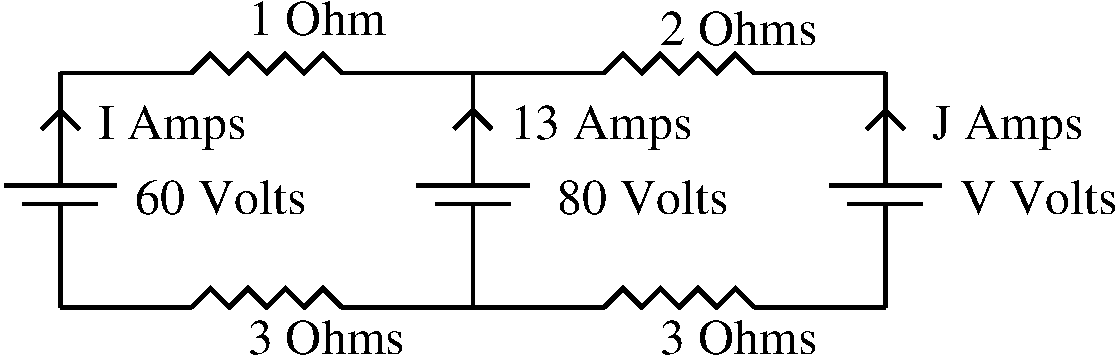
\includegraphics[scale=.6]{circuit.pdf}
$$
Find all possible equations for the unknowns $I$, $J$ and $V$ and then  solve for $I$, $J$ and $V$. Give your answers with correct units.



\item
Suppose $M$ is the matrix of a linear transformation 
$$
L: U\to V
$$
and the vector spaces $U$ and $V$ have dimensions
$$
\mbox{dim}\,  U= n\,,  \qquad \mbox{dim}\,  V= m\, , 
$$
and
$$
m\neq n\, .
$$
Also assume 
$$
\mbox{ker} L = \{0_U\}\, .
$$
\begin{enumerate}
\item How many rows does $M$ have? 
\item How many columns does $M$ have?
\item Are the columns of $M$ linearly independent?
\item What size matrix is $M^TM$?
\item What size matrix is $M M^T$?
\item Is $M^T M$ invertible?
\item is $M^T M$ symmetric? 
\item Is $M^TM$ diagonalizable?
\item  Does $M^TM$ have a zero eigenvalue?
\item Suppose $U=V$ and $\ker L\neq\{0_U\}$. Find an eigenvalue of $M$.
\item  Suppose $U=V$ and $\ker L\neq\{0_U\}$. Find $\det M$.
\end{enumerate}

\item Consider the system of equations
$$
\begin{array}{ccccccccc}
x&+&y&+&z&+&w&=&1\\
x&+&2y&+&2z&+&2w&=&1\\
x&+&2y&+&3z&+&3w&=&1\\
\end{array}
$$
Express this system as a matrix equation $MX=V$ and then find the solution set by computing an $LU$ 
decomposition for the matrix $M$ (be sure to use back and forward substitution).

\item
Compute the following determinants
$$
\det\begin{pmatrix}1&2\\3&4
\end{pmatrix},\:
\det\begin{pmatrix}1&2&3\\4&5&6\\7&8&9
\end{pmatrix},\:
\det\begin{pmatrix}1&2&3&4\\5&6&7&8\\9&10&11&12\\13&14&15&16
\end{pmatrix} ,\:$$ $$
\det\begin{pmatrix}1&2&3&4&5\\6&7&8&9&10\\11&12&13&14&15\\
16&17&18&19&20\\21&22&23&24&25
\end{pmatrix}.
$$
Now test your skills on
$$
\det\left(\begin{array}{ccccc}1&2&3&\cdots&n\\n+1&n+2&n+3&\cdots&2n\\2n+1&2n+2&2n+3&&3n \\
\vdots&&&\ddots&\vdots\\n^2-n+1&n^2-n+2&n^2-n+3&\cdots&n^2
\end{array}\right).
$$
{\it Make sure to jot down a few brief notes explaining any clever tricks you use.}

\item
For which values of $a$ does $$U={\rm span} \left\{
\begin{pmatrix}1\\0\\1\end{pmatrix},\begin{pmatrix}1\\2\\-3\end{pmatrix},\begin{pmatrix}a\\1\\0\end{pmatrix}\right\}={\mathbb R}^3\ ?$$
 For any special values of $a$ at which $U\neq{\mathbb R}^3$, express the subspace $U$ as the span of the least number of vectors possible. Give the dimension of $U$ for these cases and
 draw a picture showing $U$ inside ${\mathbb R}^3$.

\item
{\it Vandermonde determinant:}\index{Vandermonde determinant} Calculate the following determinants
$$
\det \begin{pmatrix}1 & x\\ 1 & y\end{pmatrix}\, ,\quad
\det \begin{pmatrix}1 & x & x^2\\ 1 & y&y^2\\ 1& z&z^2\end{pmatrix}\, ,\quad
\det \begin{pmatrix}1 & x & x^2 & x^3\\ 1 & y& y^2 & y^3\\ 1 & z & z^2 & z^3\\ 1 & w & w^2 & w^3\end{pmatrix}\, .
$$
Be sure to factorize you answers, if possible.

{\it Challenging:} Compute the determinant
$$
\det \begin{pmatrix}1 & x_1 & (x_1)^2 & \cdots &(x_1)^{n-1}\\ 
1 & x_2& (x_2)^2 & \cdots &  (x_2)^{n-1}\\ 
1 & x_3& (x_3)^2 & \cdots &  (x_3)^{n-1}\\ 
\vdots &\vdots &\vdots &\ddots & \vdots\ \ \  \\ 
1 & x_n& (x_n)^2 & \cdots &  (x_n)^{n-1}\end{pmatrix}\, .
$$

\item
\begin{enumerate}\item Do the vectors $\left\{\begin{pmatrix}1\\2\\3\end{pmatrix},\begin{pmatrix}3\\2\\1\end{pmatrix},\begin{pmatrix}1\\0\\0\end{pmatrix},\begin{pmatrix}0\\1\\0\end{pmatrix},\begin{pmatrix}0\\0\\1\end{pmatrix}\right\}$ form a basis for ${\mathbb R}^3$? {\it Be sure to justify your answer.}
\item
Find a basis for ${\mathbb R}^4$ that includes the vectors $\begin{pmatrix}1\\2\\3\\4\end{pmatrix}$
and $\begin{pmatrix}4\\3\\2\\1\end{pmatrix}$.
\item Explain in words how to generalize your computation in part (b) to obtain a basis for ${\mathbb R}^n$ that includes a given pair of (linearly independent) vectors $u$ and $v$. 
\end{enumerate}

\item 
Elite NASA engineers\index{Elite NASA engineers} determine that if a satellite is placed in orbit starting at a point ${\cal O}$, it will return
exactly to that same point after one orbit of the earth. Unfortunately, if there is a small mistake in the original location of the 
satellite, which the engineers label by a vector $X$ in ${\mathbb R}^3$ with origin\footnote{This is a spy satellite. The exact location of ${\cal O}$, the orientation of the coordinate axes in ${\mathbb R}^3$ and the unit system employed by the engineers are CIA secrets.} 
at~${\cal O}$, after one orbit the satellite will instead return to some other point $Y\in {\mathbb R}^3$. The engineer's computations
show that $Y$ is related to $X$ by a matrix
$$
Y = \begin{pmatrix} 0&\frac12 & 1 \\[2mm] \frac12 &\frac12 &\frac 12 \\[2mm] 1 & \frac 12 &0\end{pmatrix} X\, .
$$
\begin{enumerate}
\item Find all eigenvalues of the above matrix.
\item Determine  {\it all} possible eigenvectors associated with each eigenvalue.
\end{enumerate}
Let us assume that the rule found by the engineers applies to all subsequent orbits. 
Discuss case by case, what will happen to the satellite if the initial mistake in its location
is in a direction given by an eigenvector. 
\item
In this problem the scalars in the vector spaces are bits ($0,1$ with $1+1=0$). The space $B^k$ is the vector space of bit-valued, $k$-component column vectors.
\begin{enumerate}
\item
Find a basis for $B^3$. 
\item Your answer to part (a) should be a list of vectors $v_1$, $v_2,\ldots v_n$. What number did you find for $n$? 
\item How many elements are there in the {\it set} $B^3$. 
\item What is the dimension of the vector space $B^3$. 
\item Suppose $L:B^3\to B=\{0,1\}$ is a linear transformation. Explain why specifying $L(v_1)$, $L(v_2),\ldots,L(v_n)$ completely determines $L$. 
\item Use the notation of 
part (e) to list {all} linear transformations $$L:B^3\to B\, .$$
How many different linear transformations did you find? Compare your answer to part (c). 
\item Suppose $L_1:B^3\to B$ and $L_2: B^3\to B$ are linear transformations, and $\alpha$ and $\beta$ are bits.
Define a new map 
$(\alpha L_1+\beta L_2):B^3\to B$ by $$(\alpha L_1+\beta L_2)(v)=\alpha L_1(v)+\beta L_2(v).$$ Is this map a linear transformation? Explain.
\item Do you think the set of all linear transformations from $B^3$ to $B$ is a vector space using the addition rule above? If you answer yes, 
give a basis for this vector space and state its dimension.
\end{enumerate}

\item
A team of distinguished, post-doctoral engineers analyzes the design for a bridge across the
English channel. They notice that the force on the center of the bridge when it is displaced
by an amount $X=\begin{pmatrix}x\\y\\z\end{pmatrix}$ is given by 
$$
F=\ccolvec{-x-y\\-x-2y-z\\-y-z}\, .
$$
Moreover, having read Newton's Principi\ae\index{Newton's Principi\ae}, they know that force is proportional to acceleration so that\footnote{The bridge is intended for French and English military vehicles, so the exact units, coordinate system and constant of proportionality are state secrets.}
$$
F=\frac{d^2 X}{dt^2}\, .
$$
Since the engineers are worried the bridge might start swaying in the heavy channel winds, they search for 
an oscillatory  solution to this equation of the form\footnote{Here, $a,b,c$ and $\omega$ are constants which we aim to calculate.}
$$
X=\cos(\omega t) \ \begin{pmatrix} a \\ b \\ c\end{pmatrix}\, .
$$
\begin{enumerate}
\item By plugging their proposed solution in the above equations the engineers find an eigenvalue problem
$$
M \begin{pmatrix} a \\ b \\ c\end{pmatrix} = -\omega^2 \begin{pmatrix} a \\ b \\ c\end{pmatrix}\, .
$$
Here $M$ is a $3\times 3$ matrix. Which $3\times 3$ matrix  $M$ did the engineers find?
{\it Justify your answer.}
\item
Find the eigenvalues and eigenvectors of the matrix $M$.
\item The number $|\omega|$ is often called a {\it characteristic frequency}. What characteristic
frequencies do you find for the proposed bridge?
\item Find an orthogonal matrix $P$ such that $MP=PD$ where $D$ is a diagonal matrix.
{\it Be sure to also state your result for $D$.}
\item Is there a direction in which displacing the bridge yields no force? If so give a vector in that direction.
{\it Briefly} evaluate the quality of this bridge design.
\end{enumerate}


\item{\it Conic Sections}:\index{Conic sections} The equation for the most general conic section is given~by
$$
ax^2 + 2bxy+dy^2 + 2cx+2ey + f=0\, . 
$$
Our aim is to analyze the solutions to this equation using matrices.
\begin{enumerate}
\item \label{parta}Rewrite the above quadratic equation as one of the form $$X^T M X +  X^T C + C^T X+ f=0$$ relating an unknown column vector $X=\begin{pmatrix}x
 \\ y\end{pmatrix}$, its transpose $X^T$, a $2\times 2$ matrix $M$, a constant column vector $C$ and the  constant~$f$.
\item Does your matrix $M$ obey any special properties? Find its eigenvalues. You may call your answers $\lambda$ and $\mu$ for the rest of the problem to save writing.
\begin{quote}{\it For the rest of this problem we will focus on central conics for which the matrix $M$ is invertible.}\end{quote}
\item Your equation in part (a) above should be be quadratic in $X$. Recall that if $m\neq 0$, 
the quadratic equation $mx^2 + 2cx+f=0$ can be rewritten by {\it completing the square}
$$
m\Big(x+\frac cm\Big)^2 = \frac{c^2}{m}-f\, .
$$
Being very careful that you are now dealing with matrices, use the same trick to rewrite your answer to part (a) in the form
$$
Y^T M Y = g.
$$
Make sure you give formulas for the new unknown column vector~$Y$ and constant $g$ in terms of $X$, $M$, $C$ and $f$. You need not multiply out any of the matrix expressions you find.
\begin{quote}{\it 
If all has gone well, you have found a way to shift coordinates for the original conic equation
to a new coordinate system with its origin at the center of symmetry. Our next aim is to rotate the coordinate
axes to produce a readily recognizable equation.}
\end{quote}
\item Why is the angle between vectors $V$ and $W$ is not changed when you replace
them by $PV$ and $PW$ for $P$ any orthogonal matrix?
\item Explain how to choose an orthogonal  matrix $P$ such that $MP=PD$ where $D$ is a diagonal matrix.
\item For the choice of $P$ above, define our final unknown vector $Z$ by $Y=PZ$. Find an expression for $Y^T MY$ in terms of $Z$ and the eigenvalues of $M$.
\item Call $Z=\begin{pmatrix}z\\w\end{pmatrix}$. What equation do $z$ and $w$ obey?
(Hint, write your answer using $\lambda$, $\mu$ and $g$.)
\item Central conics are circles, ellipses, hyperbolae or a pair of straight lines. Give examples of values of 
$(\lambda,\mu,g)$ which produce each of these cases.

\end{enumerate}

\item Let \(L \colon V \to W\) be a linear transformation between finite-dimensional vector spaces \(V\) and \(W\), and let \(M\) be a matrix for \(L\) (with respect to some basis for \(V\) and some basis for \(W\)). We know that \(L\) has an inverse if and only if it is bijective, and we know a lot of ways to tell whether \(M\) has an inverse. In fact, \(L\) has an inverse if and only if \(M\) has an inverse:
\begin{enumerate}
\item Suppose that \(L\) is bijective (i.e., one-to-one and onto).
\begin{enumerate}
\item Show that \(\dim V=\rank L=\dim W\).
\item Show that \(0\) is not an eigenvalue of \(M\).
\item Show that \(M\) is an invertible matrix. 
\end{enumerate}
\item Now, suppose that \(M\) is an invertible matrix.
\begin{enumerate}
\item Show that \(0\) is not an eigenvalue of \(M\).
\item Show that \(L\) is injective.
\item Show that \(L\) is surjective.
\end{enumerate}
\end{enumerate}

\item Captain Conundrum gives Queen Quandary\index{Queen Quandary} a pair of newborn doves, male and female for her birthday. After one year, this pair of doves breed and produce a pair of dove eggs. One year later these eggs hatch yielding a new pair of doves while the original pair of doves breed again and an additional pair of eggs are laid.  Captain Conundrum is
very happy because now he will never need to buy the Queen a present ever again! 

Let us say that in year zero, the Queen has no doves. In year one she has one pair of doves, in year two she has two pairs of doves {\it etc...}
Call $F_n$ the number of pairs of doves in  years~$n$. For example, $F_0=0$, $F_1=1$ and $F_2=1$. Assume no doves die and that the same breeding pattern continues well into the future. Then $F_3=2$ because the eggs laid by the first pair of doves in year two hatch. Notice also that in year three,  two pairs of eggs are laid (by the first and second pair of doves). Thus $F_4=3$.
\begin{enumerate}
\item Compute $F_5$ and $F_6$.
\item Explain why (for any $n\geq 2$) the following {\it recursion relation}\index{Recursion relation}  holds
$$
F_n=F_{n-1}+F_{n-2}\, .
$$
\item Let us introduce a column vector
$X_n=\begin{pmatrix}\mc{F_n}\\F_{n-1}\end{pmatrix}
$. Compute $X_1$ and~$X_2$. Verify that these vectors obey the relationship
$$
X_2=M X_1 \mbox{ where } M=\begin{pmatrix}1 & 1\\1 & 0\end{pmatrix}\, . $$
\item Show that $X_{n+1}=M X_{n}$.
\item Diagonalize $M$. ({\it I.e.}, write $M$ as a product $M=PDP^{-1}$ where $D$ is diagonal.)
\item Find a simple expression for $M^n$ in terms of $P$, $D$ and $P^{-1}$.
\item Show that $X_{n+1}=M^n X_1$.
\item The number
$$\varphi=\frac{1+\sqrt{5}}2 $$
is called the {\it golden ratio}\index{Golden ratio}. Write the eigenvalues of $M$ in terms of~$\varphi$.
\item Put your results from parts (c), (f) and (g) together (along with a short matrix computation) to find
the formula for the number of doves  $F_n$ in year~$n$ expressed in terms of $\varphi$, $1-\varphi$ and $n$.
\end{enumerate}

\item
Use Gram--Schmidt to find an orthonormal basis for
$$
\mbox{span} 
\left\{
\begin{pmatrix}
1\\1\\1\\1
\end{pmatrix}\, ,\,
\begin{pmatrix}
1\\0\\1\\1
\end{pmatrix}\, ,\,
\begin{pmatrix}
0\\0\\1\\2
\end{pmatrix}
\right\}\, .
$$

\item Let $M$ be the matrix of a linear transformation $L:V\to W$ in given bases for $V$ and $W$.
Fill in the blanks below with one of the following six vector spaces: $V$, $W$, ${\rm ker} L$, 
$\big({\rm ker} L\big)^\perp$, ${\rm im} L$, $\big({\rm im} L\big)^\perp$.
\begin{enumerate}
\item The columns of $M$ span \underline{\phantom{answer}} in the basis given for \underline{\phantom{answer}}.
\item The rows of $M$ span \underline{\phantom{answer}} in the basis given for \underline{\phantom{answer}}.
\end{enumerate} 
Suppose $$M=\begin{pmatrix}1&2&1&3\\2&1&\!-1&2\\1&0&0&\!-1\\4&1&\!-1&0\end{pmatrix}$$
is the matrix of $L$ in the bases $\{v_1,v_2,v_3,v_4\}$ for $V$ and $\{w_1,w_2,w_3,w_4\}$ for~$W$.
Find bases for ${\rm ker} L$ and ${\rm im} L$. Use the dimension formula to check your result.

\item
Captain Conundrum collects the following data set
$$
\begin{array}{c|c}
y&x\\
\hline
5&-2\\
2&-1\\
0&1\\
3&2
\end{array}
$$
which he believes to be well-approximated by a parabola
$$
y=ax^2+bx+c\, .
$$

\begin{enumerate}
\item Write down a system of four linear equations for the unknown coefficients $a$, $b$ and $c$.
\item Write the augmented matrix for this system of equations.
\item Find the reduced row echelon form for this augmented matrix.
\item Are there any solutions to this system?
\item Find the least squares solution to the system.
\item What value does Captain Conundrum predict for $y$ when $x=2$? 
\end{enumerate}


\item Suppose you have collected the following data for an experiment
$$
\begin{array}{l|l}
x&y\\\hline
x_1&y_1\\
x_2&y_2\\
x_3&y_3
\end{array}
$$
and believe that the result is well modeled by a straight line
$$
y=mx+b\, .
$$
\begin{enumerate}
\item Write down a linear system of equations you could use to find the slope $m$ and constant term~$b$. 
\item Arrange the unknowns $(m,b)$ in a column vector $X$ and write your answer to (a) as a matrix equation $$M X= V\, .$$
Be sure to give explicit expressions for the matrix $M$ and column vector $V$.
\item For a generic data set, would you expect your system of equations to have a solution? {\it Briefly} explain your answer.
\item Calculate $M^T M$ and $(M^T M)^{-1}$ (for the latter computation, state the condition required for the inverse to exist).
\item Compute the least squares solution for $m$ and $b$.
\item The least squares method determines a vector $X$ that minimizes the length of the vector $V-MX$. Draw a rough sketch of
the three data points in the $(x,y)$-plane as well as their least squares fit. 
Indicate how the components of $V-MX$ could be obtained from your picture.

\end{enumerate}

\end{enumerate}

\subsection*{Solutions}

\begin{enumerate}
\item You can find the definitions for all these terms by consulting the index of this book.

\item Both junctions give the same equation for the currents
$$
I+J+13=0\, .
$$
There are three voltage loops (one on the left, one on the right and one going around the outside of the circuit). Respectively, they give the equations
\begin{eqnarray}
&60-I-80-3I=0&\nn\\[2mm]
&80+2J-V+3J=0&\nn\\[2mm]
&60-I+2J-V+3J-3I=0&\, .
\end{eqnarray}
The above equations are easily solved (either using an augmented matrix and row reducing, or by substitution). The result is $I=-5$ Amps, $J=-8$ Amps, $V=40$ Volts.



\item 
\begin{enumerate}
\item $m$.
\item $n$.
\item Yes.
\item $n\times n$.
\item $m\times m$.
\item Yes. This relies on ${\rm ker} M=0$ because if $M^T M$ had a non-trivial kernel, then there would be a non-zero solution $X$ to $M^T M X=0$. But then by multiplying on the left by $X^T$ we see that $||MX||=0$. This in turn implies $MX=0$ which contradicts the triviality of the kernel of $M$. 
\item Yes because $\big(M^T M\big)^T=M^T (M^T)^T=M^T M$.
\item Yes, all symmetric matrices have a basis of eigenvectors.
\item No, because otherwise it would not be invertible.
\item Since the kernel of $L$ is non-trivial, $M$ must have $0$ as an eigenvalue.
\item Since $M$ has a zero eigenvalue in this case, its determinant must vanish. {I.e.}, $\det M=0$.
\end{enumerate}

\item To begin with the system becomes
$$
\begin{pmatrix}1&1&1&1\\[1mm]1&2&2&2\\[1mm]1&2&3&3
\end{pmatrix}
\begin{pmatrix}x\\[1mm]y\\[1mm]z\\[1mm]w\end{pmatrix}=
\begin{pmatrix}1\\[1mm]1\\[1mm]1\end{pmatrix}
$$
Then
$$
M=
\begin{pmatrix}
1&1&1&1\\[1mm]1&2&2&2\\[1mm]1&2&3&3
\end{pmatrix}
=
\begin{pmatrix}
1&0&0\\[1mm]1&1&0\\[1mm]1&0&1
\end{pmatrix}
\begin{pmatrix}
1&1&1&1\\[1mm]0&1&1&1\\[1mm]0&1&2&2
\end{pmatrix}$$ $$
=
\begin{pmatrix}
1&0&0\\[1mm]1&1&0\\[1mm]1&1&1
\end{pmatrix}
\begin{pmatrix}
1&1&1&1\\[1mm]0&1&1&1\\[1mm]0&0&1&1
\end{pmatrix}=LU
$$
So now $MX=V$ becomes $LW=V$ where $W=UX=\begin{pmatrix}a\\b\\c\end{pmatrix}$ (say). Thus we solve $LW=V$ by forward substitution
$$
a=1,\ a+b=1,  \ a+b+c=1 \Rightarrow a=1,b=0,c=0\, .
$$
Now solve $UX=W$ by back substitution
$$
x+y+z+w=1, \ y+z+w=0, \ z + w =0$$ $$ \ \Rightarrow
w=\mu \mbox{ (arbitrary)}, z=-\mu, y=0, x=1\, .
$$
The solution set is $\left\{\begin{pmatrix}x\\y\\z\\y\end{pmatrix}=\begin{pmatrix}1\\0\\-\mu\\\mu\end{pmatrix}: \mu\in {\mathbb R}\right\}$


\item First 
$$\det\begin{pmatrix}1&2\\3&4\end{pmatrix}=-2\, .$$
All the other determinants vanish because the first three rows of each matrix are not independent. 
Indeed, $2R_2-R_1=R_3$ in each case, so we can make row operations to get a row of zeros and thus a zero determinant. 

\item If $U$ spans ${\mathbb R}^3$, then we must be able to express any vector $X=\begin{pmatrix}x\\y\\z\end{pmatrix}$ $\in {\mathbb R}^3$
as
$$
X=c^1\begin{pmatrix}1\\0\\1\end{pmatrix}+c^2\begin{pmatrix}1\\2\\-3\end{pmatrix}+c^3\begin{pmatrix}a\\1\\0\end{pmatrix}
=\begin{pmatrix}1&1&a\\0&2&1\\1&-3&0\end{pmatrix}\begin{pmatrix}c^1\\c^2\\c^3\end{pmatrix}\, ,
$$
for some coefficients $c^1$, $c^2$ and $c^3$. This is a linear system. We could solve for $c^1$, $c^2$ and $c^3$ using an
augmented matrix and row operations. However, since we know that ${\rm dim}\, {\mathbb R}^3=3$, if $U$ spans ${\mathbb R}^3$,
it will also be a basis. Then the solution for  $c^1$, $c^2$ and $c^3$ would be unique. Hence, the $3\times 3$ matrix above must 
be invertible, so we examine its determinant
$$
{\rm det} \begin{pmatrix}1&1&a\\0&2&1\\1&-3&0\end{pmatrix}
=1.(2.0-1.(-3))+1.(1.1-a.2)=4-2a\, .
$$
Thus $U$ spans ${\mathbb R}^3$ whenever $a\neq 2$. When $a=2$ we can write the third vector in $U$ in terms of the preceding ones as
$$
\begin{pmatrix}2\\1\\0\end{pmatrix}=\frac32\begin{pmatrix}1\\0\\1\end{pmatrix}+\frac12\begin{pmatrix}1\\2\\-3\end{pmatrix}.
$$
({\it You can obtain this result, or an equivalent one by studying the above linear system with $X=0$, i.e., the associated homogeneous system.}) The two vectors $\begin{pmatrix}1\\2\\-3\end{pmatrix}$ and $\begin{pmatrix}2\\1\\0\end{pmatrix}$ are clearly linearly independent,
so this is the least number of vectors spanning $U$ for this value of $a$. Also we see that dim$U=2$ in this case. Your picture should be
a plane in ${\mathbb R}^3$ though the origin  containing the vectors $\begin{pmatrix}1\\2\\-3\end{pmatrix}$ and $\begin{pmatrix}2\\1\\0\end{pmatrix}$.

\item 
$$
\det \begin{pmatrix}1 & x\\ 1 & y\end{pmatrix}=y-x\, ,\ \ 
$$

$$
\det \begin{pmatrix}1 & x & x^2\\ 1 & y&y^2\\ 1& z&z^2\end{pmatrix}=
\det \begin{pmatrix}1 & x & x^2\\ 0 & y-x&y^2-x^2\\ 0& z-x&z^2-x^2\end{pmatrix}$$ $$
=(y-x)(z^2-x^2)-(y^2-x^2)(z-x)=(y-x)(z-x)(z-y)\, .
$$

$$
\det \begin{pmatrix}1 & x & x^2 & x^3\\ 1 & y& y^2 & y^3\\ 1 & z & z^2 & z^3\\ 1 & w & w^2 & w^3\end{pmatrix}
=
\det \begin{pmatrix}1 & x & x^2 & x^3\\ 0 & y-x& y^2-x^2 & y^3-x^3\\ 0 & z-x & z^2 -x^2& z^3-x^3\\ 0 & w-x & w^2-x^2 & w^3-x^3\end{pmatrix}
$$
$$
=
\det \begin{pmatrix}1 & 0 & 0 & 0\\ 0 & y-x& y(y-x)& y^2(y-x)\\ 0 & z-x & z(z-x) & z^2(z-x)\\ 0 & w-x & w(w-x) & w^2(w-x)\end{pmatrix}
$$
$$=
(y-x)(z-x)(w-x)\det \begin{pmatrix}1 & 0 & 0 & 0\\ 0 & 1& y& y^2\\ 0 & 1 & z & z^2\\ 0 & 1 & w & w^2\end{pmatrix}
$$
$$
=(y-x)(z-x)(w-x)\det \begin{pmatrix}1 & y & y^2\\ 1 & z&z^2\\ 1& w&w^2\end{pmatrix}
$$
$$
=(y-x)(z-x)(w-x) (z-y)(w-y)(w-z)\, .
$$
From the $4\times 4$ case above, you can see all the tricks required for a general Vandermonde matrix.
First zero out the first column by subtracting the first row from all other rows (which leaves the determinant unchanged). Now zero out the top row by subtracting $x_1$ times the first column from the second column,
$x_1$ times the second column from the third column {\it et cetra}. Again these column operations do not
change the determinant. Now factor out $x_2-x_1$ from the second row, $x_3-x_1$ from the third row, {\it etc}. This does change the determinant so we write these factors outside the remaining determinant, which is just the same problem but for the $(n-1)\times(n-1)$ case. Iterating the same procedure gives the result
$$
\det \begin{pmatrix}1 & x_1 & (x_1)^2 & \cdots &(x_1)^{n-1}\\ 
1 & x_2& (x_2)^2 & \cdots &  (x_2)^{n-1}\\ 
1 & x_3& (x_3)^2 & \cdots &  (x_3)^{n-1}\\ 
\mc\vdots &\mc\vdots &\mc\vdots &\ddots & \mc\vdots\ \ \  \\ 
1 & x_n& (x_n)^2 & \cdots &  (x_n)^{n-1}\end{pmatrix}
=\prod_{i>j}(x_i-x_j)\, .
$$
(Here $\prod$ stands for a multiple product, just like $\Sigma$ stands for a multiple sum.)

\item \begin{enumerate}
\item No, a basis for  ${\mathbb R}^3$ must have exactly three vectors.
\item We first extend the original vectors by the standard basis for ${\mathbb R}^4$ and then try to eliminate two of them by considering
$$
\alpha \begin{pmatrix}1\\2\\3\\4\end{pmatrix}+\beta
\begin{pmatrix}4\\3\\2\\1\end{pmatrix} +\gamma 
\begin{pmatrix}1\\0\\0\\0\end{pmatrix}
+\delta\begin{pmatrix}0\\1\\0\\0\end{pmatrix}
+\varepsilon\begin{pmatrix}0\\0\\1\\0\end{pmatrix}
+\eta\begin{pmatrix}0\\0\\0\\1\end{pmatrix}=0\, .
$$ 
So we study
$$
\begin{pmatrix}
1&4&1&0&0&0\\
2&3&0&1&0&0\\
3&2&0&0&1&0\\
4&1&0&0&0&1
\end{pmatrix}
\sim
\begin{pmatrix}
1&4&1&0&0&0\\
0&-5&-2&1&0&0\\
0&-10&-3&0&1&0\\
0&-15&-4&0&0&1
\end{pmatrix}
$$
$$
\sim
\begin{pmatrix}
1&0&-\frac35&-4&0&0\\
0&1&\frac25&\frac15&0&0\\[1mm]
0&0&1&10&1&0\\
0&0&2&15&0&1
\end{pmatrix}
\sim
\begin{pmatrix}
1&0&0&2&\frac35&0\\
0&1&0&-\frac{19}5&-\frac25&0\\[1mm]
0&0&1&10&1&0\\
0&0&0&-\frac{5}2&-10&\frac12
\end{pmatrix}
$$
From here we can keep row reducing to achieve RREF, but we can already see that the non-pivot variables will be
$\varepsilon$ and $\eta$. Hence we can eject the last two vectors and obtain as our basis
$$
\left\{
\begin{pmatrix}1\\2\\3\\4\end{pmatrix},
\begin{pmatrix}4\\3\\2\\1\end{pmatrix},
\begin{pmatrix}1\\0\\0\\0\end{pmatrix},
\begin{pmatrix}0\\1\\0\\0\end{pmatrix}
\right\}\, .
$$
Of course, this answer is far from unique!
\item The method is the same as above. Add the standard basis to $\{u,v\}$ to obtain the linearly dependent set
$\{u,v,e_1,\ldots , e_n\}$. Then put these vectors as the columns of a matrix and row reduce. The  standard basis
vectors in columns corresponding to the non-pivot variables can be removed.
\end{enumerate}


\item 
\begin{enumerate}
\item
$$
{\rm det} \begin{pmatrix} \lambda&-\frac12 & -1 \\[2mm] -\frac12 &\lambda-\frac12 &-\frac12 \\[2mm] -1 & -\frac12 &\lambda\end{pmatrix}
=\lambda\Big((\lambda-\frac12\Big)\lambda-\frac14)+\frac12\Big(-\frac{\lambda}2-\frac12\Big)-\Big(-\frac14+\lambda\Big)
$$
$$
=\lambda^3-\frac{1}{2}\lambda^2-\frac32 \lambda=\lambda(\lambda+1)(\lambda-\frac32)\, .
$$
Hence the eigenvalues are $0,-1,\frac32$.
\item
When $\lambda=0$ we must solve the homogenous system
$$
\left(
\begin{array}{ccc|c}
0&\frac12&1&0\\[1mm]
\frac12&\frac12&\frac12&0\\[1mm]
1&\frac12&0&0
\end{array}\right)
\sim
\left(
\begin{array}{ccc|c}
1&\frac12&0&0\\[1mm]
0&\frac14&\frac12&0\\[1mm]
0&\frac12&1&0
\end{array}\right)
\sim
\left(
\begin{array}{ccc|c}
1&0&-1&0\\[1mm]
0&1&2&0\\[1mm]
0&0&0&0
\end{array}\right)\, .
$$
So we find the eigenvector $\begin{pmatrix}s\\-2s\\s\end{pmatrix}$ where $s\neq 0$ is arbitrary.

For $\lambda=-1$ 
$$
\left(
\begin{array}{ccc|c}
1&\frac12&1&0\\[1mm]
\frac12&\frac32&\frac12&0\\[1mm]
1&\frac12&1&0
\end{array}\right)
\sim
\left(
\begin{array}{ccc|c}
1&0&1&0\\[1mm]
0&1&0&0\\[1mm]
0&0&0&0
\end{array}\right)
\, .
$$
So we find the eigenvector $\begin{pmatrix}-s\\0\\s\end{pmatrix}$ where $s\neq 0$ is arbitrary.

Finally, for $\lambda=\frac32$
$$
\left(
\begin{array}{ccc|c}
-\frac32&\frac12&1&0\\[1mm]
\frac12&-1&\frac12&0\\[1mm]
1&\frac12&-\frac32&0
\end{array}\right)
\sim
\left(
\begin{array}{ccc|c}
1&\frac12&-\frac32&0\\[1mm]
0&-\frac54&\frac54&0\\[1mm]
0&\frac54&-\frac54&0
\end{array}\right)
\sim
\left(
\begin{array}{ccc|c}
1&0&-1&0\\[1mm]
0&1&-1&0\\[1mm]
0&0&0&0
\end{array}\right)\, .
$$
So we find the eigenvector $\begin{pmatrix}s\\s\\s\end{pmatrix}$ where $s\neq 0$ is arbitrary.
\end{enumerate}
If the mistake $X$ is in the direction of the eigenvector $\begin{pmatrix}1\\-2\\1\end{pmatrix}$,
then $Y=0$. {\it I.e.}, the satellite returns to the origin ${\cal O}$. For all subsequent orbits it will again return to 
the origin. NASA would be very pleased in this case.

If the mistake $X$ is in the direction $\begin{pmatrix}-1\\0\\1\end{pmatrix}$, then $Y=-X$. Hence the satellite will move to the point opposite to $X$. After next orbit will move back to $X$. It will continue this wobbling
motion indefinitely. Since this is a stable situation, again, the elite engineers will pat themselves on the back.

Finally, if the mistake  $X$ is in the direction $\begin{pmatrix}1\\1\\1\end{pmatrix}$ , the satellite will move
to a point $Y=\frac32 X$ which is further away from the origin. The same will happen for all subsequent
orbits, with the satellite moving a factor $3/2$ further away from ${\cal O}$ each orbit (in reality, after
several orbits, the approximations used by the engineers in their calculations probably fail and a new computation  will be needed). In this case, the satellite will be lost in outer space and the engineers will likely lose their jobs!

\item 
\begin{enumerate}
\item A basis for $B^3$ is $\left\{
\begin{pmatrix}1\\0\\0\end{pmatrix},
\begin{pmatrix}0\\1\\0\end{pmatrix},
\begin{pmatrix}0\\0\\1\end{pmatrix}
\right\}$
\item 3.
\item $2^3=8$.
\item dim$B^3=3$.
\item Because the vectors $\{v_1,v_2,v_3\}$ are a basis any element $v\in B^3$ can be
written uniquely as $v=b^1 v_1 +b^2 v_2+b^3 v_3$ for some triplet of bits~$\begin{pmatrix}b^1\\b^2\\b^3\end{pmatrix}$. Hence, to compute $L(v)$ we use linearity of $L$
$$
L(v) = L(b^1 v_1 +b^2 v_2+b^3 v_3) = b^1 L(v_1)  + b^2 L(v_2) + b^3 L(v_3) $$ $$= \begin{pmatrix}L(v_1) & L(v_2) & L(v_3)\end{pmatrix}
\begin{pmatrix}b^1\\b^2\\b^3\end{pmatrix}\, .
$$
\item From the notation of the previous part, we see that we can list  linear transformations $L:B^3\to B$
by writing out all possible bit-valued row vectors
\begin{eqnarray*}
&\begin{pmatrix}0 & 0 & 0\end{pmatrix} ,\\
&\begin{pmatrix}1 & 0 & 0\end{pmatrix} ,\\
&\begin{pmatrix}0 & 1 & 0\end{pmatrix} ,\\
&\begin{pmatrix}0 & 0 & 1\end{pmatrix} ,\\
&\begin{pmatrix}1 & 1 & 0\end{pmatrix} ,\\
&\begin{pmatrix}1 & 0 & 1\end{pmatrix} ,\\
&\begin{pmatrix}0 & 1 & 1\end{pmatrix} ,\\
&\begin{pmatrix}1 & 1  & 1\end{pmatrix} .
\end{eqnarray*}
There are $2^3=8$ different linear transformations $L:B^3\to B$, exactly the same as the number of elements in $B^3$.
\item Yes, essentially just because $L_1$ and $L_2$ are linear transformations. In detail for any bits
$(a,b)$ and vectors $(u,v)$ in $B^3$ it is easy to check the linearity property for $(\alpha L_1+\beta L_2)$
$$(\alpha L_1+\beta L_2)(a u + b v)=\alpha L_1(a u + b v)+\beta L_2(au + bv) 
$$
$$
=\alpha a L_1(u) + \alpha b L_1(v)+ \beta a L_1(u) + \beta b L_1(v) 
$$ $$= a (\alpha L_1(u) + \beta L_2(v))
+ b (\alpha L_1(u) + \beta L_2(v))
$$
$$
=a (\alpha L_1 + \beta L_2)(u) + b  (\alpha L_1 + \beta L_2)(v)\, .
$$
Here the first line used the definition of $(\alpha L_1 + \beta L_2)$, the second line depended on
the linearity of $L_1$ and $L_2$, the third line was just algebra and the fourth used the definition of $(\alpha L_1+ \beta L_2)$ again.
\item Yes. The easiest way to see this is the identification above of these maps with bit-valued column vectors. In that notation, a basis is 
$$\Big\{\begin{pmatrix}1&0&0\end{pmatrix},\begin{pmatrix}0&1&0\end{pmatrix},\begin{pmatrix}0&0&1\end{pmatrix}\Big\}\, .$$
Since this (spanning) set has three (linearly independent) elements, the vector space of linear maps $B^3\to B$ has dimension~3. This is an example of a general notion called the {\it dual vector space}\index{Dual vector space}.\end{enumerate}

\item 
\begin{enumerate}
\item $\frac{d^2 X}{dt^2}=\frac{d^2\cos(\omega t )}{dt^2}\colvec{a\\b\\c}=-\omega^2\cos(\omega t) \colvec{a\\b\\c}\, .$ 

Hence
\begin{eqnarray*}
F=\cos(\omega t) \ccolvec{-a-b\\-a-2b-c\\-b-c}&=&\cos(\omega t) \begin{pmatrix}-1&-1&0\\-1&-2&-1\\0&-1&-1\end{pmatrix}\colvec{a\\b\\c}
\\[1mm]&=&-\omega^2\cos(\omega t) \colvec{a\\b\\c}
\, ,\end{eqnarray*}
so 
$$
M=\begin{pmatrix}-1&-1&0\\-1&-2&-1\\0&-1&-1\end{pmatrix}\, .
$$
\item
\begin{eqnarray*}
\det \begin{pmatrix}\lambda+1&\mc1&\mc0\\\mc1&\lambda+2&\mc1\\\mc0&\mc1&\lambda+1\end{pmatrix}
&=&(\lambda+1)\big((\lambda+2)(\lambda+1)-1\big)-(\lambda+1)\\
&=&(\lambda+1)\big((\lambda+2)(\lambda+1)-2\big)\\
&=&(\lambda+1)\big(\lambda^2+3\lambda)=\lambda(\lambda+1)(\lambda+3)\end{eqnarray*}
so the eigenvalues are $\lambda=0,-1 ,-3 $.

For the eigenvectors, when $\lambda=0$ we study:
$$
M-0.I=\begin{pmatrix}-1&-1&0\\-1&-2&-1\\0&-1&-1\end{pmatrix}\sim\begin{pmatrix}1&1&0\\0&-1&-1\\0&-1&-1\end{pmatrix}
\sim\begin{pmatrix}1&0&\!-1\\0&1&1\\0&0&0\end{pmatrix}\, ,
$$
so $\colvec{1\\-1\\1}$ is an eigenvector.

For $\lambda=-1$
$$
M-(-1).I=\begin{pmatrix}0&-1&0\\-1&-1&-1\\0&-1&0\end{pmatrix}\sim\begin{pmatrix}1&0&1\\0&1&0\\0&0&0\end{pmatrix}
\, ,
$$
so $\colvec{-1\\0\\1}$ is an eigenvector.

For $\lambda=-3$
$$
M-(-3).I=\begin{pmatrix}2&-1&0\\-1&1&-1\\0&-1&2\end{pmatrix}\sim\begin{pmatrix}1&-1&1\\0&1&-2\\0&-1&2\end{pmatrix}
\sim\begin{pmatrix}1&0&-1\\0&1&-2\\0&0&0\end{pmatrix}\, ,
$$
so $\colvec{1\\2\\1}$ is an eigenvector.

\item The characteristic frequencies are $0,1,\sqrt{3}$.
\item The orthogonal change of basis matrix 
$$
P=\begin{pmatrix}
\frac1{\sqrt{3}}&-\frac1{\sqrt{2}}&\frac{1}{\sqrt{6}}\\
-\frac1{\sqrt{3}}&\mc 0&\frac{2}{\sqrt{6}}\\
\frac1{\sqrt{3}}&\frac1{\sqrt{2}}&\frac{1}{\sqrt{6}}
\end{pmatrix}
$$
It obeys $MP=PD$ where
$$
D=\begin{pmatrix}0&0&0\\0&-1&0\\0&0&-3\end{pmatrix}\, .
$$
\item Yes, the direction given by the eigenvector $\colvec{1\\-1\\1}$ because its eigenvalue is zero. This is probably a bad design for a bridge because it can be displaced in this direction with no force!
\end{enumerate}

\item 
\begin{enumerate}
\item If we call $M=\begin{pmatrix}a&b\\b&d\end{pmatrix}$, then $X^TMX=ax^2 + 2bxy + dy^2$.
Similarly putting $C=\begin{pmatrix}c\\e\end{pmatrix}$ yields $X^T C + C^T X = 2 X \dotprod C = 2 cx + 2 e y$. Thus
$$
0=
ax^2 + 2bxy + dy^2+2cx+2ey+f$$
$$=\begin{pmatrix} x & y\end{pmatrix} \begin{pmatrix}a&b\\b&d\end{pmatrix}
\begin{pmatrix} x \\ y\end{pmatrix}+ 
\begin{pmatrix} x & y\end{pmatrix}\begin{pmatrix}c\\e\end{pmatrix}+
\begin{pmatrix} c & e\end{pmatrix}\begin{pmatrix}x\\y\end{pmatrix}+f\, .
$$
\item Yes, the matrix $M$ is symmetric, so it will have a basis of eigenvectors and is similar to
a diagonal matrix of real eigenvalues.

To find the eigenvalues notice that $\det\begin{pmatrix}a-\lambda&b\\b&d-\lambda\end{pmatrix}
=(a-\lambda)(d-\lambda)-b^2=\big(\lambda-\frac{a+d}{2}\big)^2-b^2-\big(\frac{a-d}{2}\big)^2$.
So the eigenvalues are $$\lambda=\frac{a+d}{2}+\sqrt{b^2+\big(\frac{a-d}{2}\big)^2}
\mbox{ and } \mu=\frac{a+d}{2}-\sqrt{b^2+\big(\frac{a-d}{2}\big)^2}\, .$$
\item The trick is to write
$$X^T M X + C^T X + X^T C =(X^T+C^T M^{-1}) M (X+M^{-1} C) - C^T M^{-1} C\, ,$$
so that
$$(X^T+C^T M^{-1}) M (X+M^{-1} C) = C^T M C -f\, .$$
Hence $Y=X+M^{-1} C$ and $g=C^T M C -f$.
\item The cosine of the angle between vectors $V$ and $W$ is given by $$\frac{V\dotprod W}{\sqrt{V\dotprod V\, W\dotprod W}}=\frac{V^T W}{\sqrt{V^T V\, W^T W}}\, .$$ 
So replacing $V\to PV$ and $W\to PW$ will always give a factor $P^T P$ inside all the products, but $P^TP=I$ for orthogonal matrices. Hence none of the dot products in the above formula changes, so 
neither does the angle between $V$ and $W$.
\item If we take the eigenvectors of $M$, normalize them ({\it i.e.} divide them by their lengths),
and put them in a matrix $P$ (as columns) then $P$ will be an orthogonal matrix. (If it happens
that $\lambda=\mu$, then we also need to make sure the eigenvectors spanning the two dimensional
eigenspace corresponding to $\lambda$ are orthogonal.) Then, since $M$ times the eigenvectors
yields just the eigenvectors back again multiplied by their eigenvalues, it follows that $MP=PD$
where $D$ is the diagonal matrix made from eigenvalues.
\item If $Y=PZ$, then $Y^T M Y= Z^T P^T M P Z = Z^T P^T P D Z = Z^T D Z$ where $D=\begin{pmatrix}\lambda & 0 \\ 0&\mu \end{pmatrix}$.
\item Using part (f) and (c) we have 
$$\lambda z^2 + \mu w^2 = g\, .$$
\item When $\lambda=\mu$ and $g/\lambda=R^2$, we get the equation for a circle radius $R$ in the $(z,w)$-plane. When $\lambda$, $\mu$ and $g$ are postive, we have the equation for an ellipse. Vanishing $g$ along with $\lambda$ and $\mu$ of opposite signs gives a pair of straight lines.
When $g$ is non-vanishing, but $\lambda$ and $\mu$ have opposite signs, the result is a pair of hyperbol\ae. These shapes all come from cutting a cone with a plane, and are therefore called
conic sections.
\end{enumerate}

\item  We  show  that  \(L\)  is  bijective  if  and  only  if  \(M\)  is  invertible.
 		\begin{enumerate}
 		\item  We  suppose  that  \(L\)  is  bijective.
 		\begin{enumerate}
 		\item  Since  \(L\)  is  injective,  its  kernel  consists  of  the  zero  vector  alone.  Hence
 		\[
 		\null  L=\dim  \ker  L=0.
 		\]
 		So  by  the  Dimension  Formula,
 		\[
 		\dim  V=\null  L+\rank  L=\rank  L.
 		\]
 		Since  \(L\)  is  surjective,  \(L(V)=W.\)  Thus
 		\[
 		\rank  L=\dim  L(V)=\dim  W.
 		\]
 		Thereby  \[\dim  V=\rank  L=\dim  W.\]
 		\item  Since  \(\dim  V=\dim  W\),  the  matrix  \(M\)  is  square  so  we  can  talk  about  its  eigenvalues.  Since  \(L\)  is  injective,  its  kernel  is  the  zero  vector  alone.  That  is,  the  only  solution  to  \(LX=0\)  is  \(X=0_V\).  But  \(LX\)  is  the  same  as  \(MX\),  so  the  only  solution  to  \(MX=0\)  is  \(X=0_V\).  So  \(M\)  does  not  have  zero  as  an  eigenvalue.
 		\item  Since  \(MX=0\)  has  no  non-zero  solutions,  the  matrix  \(M\)  is  invertible.
	\end{enumerate}
 		\item  Now  we  suppose  that  \(M\)  is  an  invertible  matrix.
 		\begin{enumerate}
 		\item  Since  \(M\)  is  invertible,  the  system  \(MX=0\)  has  no  non-zero  solutions.  But  \(LX\)  is  the  same  as  \(MX\),  so  the  only  solution  to  \(LX=0\)  is  \(X=0_V\).  So  \(L\)  does  not  have  zero  as  an  eigenvalue.
 		\item  Since  \(LX=0\)  has  no  non-zero  solutions,  the  kernel  of  \(L\)  is  the  zero  vector  alone.  So  \(L\)  is  injective.
 		\item  Since  \(M\)  is  invertible,  we  must  have  that  \(\dim  V=\dim  W\).  By  the  Dimension  Formula,  we  have
 		\[
 		\dim  V=\null  L+\rank  L
 		\]
 		and  since  \(\ker  L=\{0_V\}\)  we  have  \(\null  L=\dim  \ker  L=0\),  so
 		\[
 		\dim  W=\dim  V=\rank  L=\dim  L(V).
 		\]
 		Since  \(L(V)\)  is  a  subspace  of  \(W\)  with  the  same  dimension  as  \(W\),  it  must  be  equal  to  \(W\).  To  see  why,  pick  a  basis  \(B\)  of  \(L(V)\).  Each  element  of  \(B\)  is  a  vector  in  \(W\),  so  the  elements  of  \(B\)  form  a  linearly  independent  set  in  \(W\).  Therefore  \(B\)  is  a  basis  of  \(W\),  since  the  size  of  \(B\)  is  equal  to  \(\dim  W\).  So  \(L(V)=\spa  B=W.\)  So  \(L\)  is  surjective.
 		\end{enumerate}
 		\end{enumerate}

\item 
\begin{enumerate}
\item $F_4=F_2+F_3=2+3=5$.
\item The number of pairs of doves in any given year equals the number of the previous years plus those that hatch and there are as many of them as pairs of doves in the year before the previous year.
\item $X_1=\begin{pmatrix}F_1\\F_0\end{pmatrix}=\begin{pmatrix}1\\0\end{pmatrix}$
and $X_2=\begin{pmatrix}F_2\\F_1\end{pmatrix}=\begin{pmatrix}1\\1\end{pmatrix}$.
$$
MX_1=\begin{pmatrix}1 & 1\\ 1& 0\end{pmatrix}\begin{pmatrix}1\\ 0\end{pmatrix}
=\begin{pmatrix}1\\1\end{pmatrix}=X_2\, .
$$
\item We just need to use the recursion relationship of part (b) in the top slot of $X_{n+1}$:
$$
X_{n+1}=\ccolvec{F_{n+1}\\F_n}
=\ccolvec{F_{n}+F_{n-1}\\F_n}=
\begin{pmatrix}1 & 1\\ 1& 0\end{pmatrix}\ccolvec{F_{n}\\F_{n-1}}=M X_n\, .
$$
\item Notice $M$ is symmetric so this is guaranteed to work. $$\det \begin{pmatrix}1-\lambda&\mc1\\\mc1&-\lambda\end{pmatrix}=\lambda(\lambda-1)-1=\big(\lambda-\frac12\big)^2-\frac54\, ,$$
so the eigenvalues are $\frac{1\pm\sqrt{5}}{2}$. Hence the eigenvectors are $\ccolvec{\frac{1\pm\sqrt{5}}{2}\\1}$, respectively (notice that $\frac{1+\sqrt{5}}{2}+1=\frac{1+\sqrt{5}}{2}.\frac{1+\sqrt{5}}{2}$ and $\frac{1-\sqrt{5}}{2}+1=\frac{1-\sqrt{5}}{2}.\frac{1-\sqrt{5}}{2}$).
Thus $M=PDP^{-1}$ with $$D=\begin{pmatrix}\frac{1+\sqrt{5}}{2}&\mc0\\[1mm]\mc0&\frac{1-\sqrt{5}}{2}\end{pmatrix} \mbox{ and } P =\begin{pmatrix}\frac{1+\sqrt{5}}{2}&\frac{1-\sqrt{5}}{2}\\[1mm]\mc1&\mc1\end{pmatrix}\, .$$
\item $M^n=(P D P^{-1})^n = P D P^{-1} P D P^{-1} \ldots P D P^{-1} = P D^n P^{-1}$.
\item Just use the matrix recursion relation of part (d) repeatedly: $$X_{n+1}= M X_{n} = M^2 X_{n-1}=\cdots = M^{n} X_1\, .$$
\item The eigenvalues are $\varphi = \frac{1+\sqrt{5}}{2}$ and $1-\varphi = \frac{1-\sqrt{5}}{2}$.
\item $$X_{n+1}=\ccolvec{F_{n+1}\\F_n}=
M^n X_n = P D^n P^{-1} X_{1}$$ $$=P 
\begin{pmatrix}\varphi&\mc0\\\mc0&1-\varphi\end{pmatrix}^{\!n} 
\begin{pmatrix}\frac{1}{\sqrt{5}}&\star \\-\frac{1}{\sqrt{5}}& \star\end{pmatrix}
\begin{pmatrix}1\\ 0\end{pmatrix}
=P 
\begin{pmatrix}\varphi^n&\mc0\\\mc0&(1-\varphi)^n\end{pmatrix}
\begin{pmatrix}\frac{1}{\sqrt{5}}\\-\frac{1}{\sqrt{5}}\end{pmatrix}
$$
$$
=\begin{pmatrix}\frac{1+\sqrt{5}}{2}&\frac{1-\sqrt{5}}{2}\\[1mm]\mc1&\mc1\end{pmatrix}
\begin{pmatrix}\mc{\frac{\varphi^n}{\sqrt{5}}}\\[1mm]-\frac{(1-\varphi)^n}{\sqrt{5}}\end{pmatrix}
=\begin{pmatrix}\mc\star \\[1mm]\frac{\varphi^n-(1-\varphi)^n}{\sqrt{5}}\end{pmatrix}.
$$
Hence
$$F_n=\frac{\varphi^n-(1-\varphi)^n}{\sqrt{5}}\, .$$
These are the famous Fibonacci numbers\index{Fibonacci numbers}.
\end{enumerate}


\item Call the three vectors $u,v$ and $w$, respectively. Then
$$
v^\perp=v-\frac{u\dotprod v}{u\dotprod u} u =v-\frac34 u = \begin{pmatrix}\frac14 \\[1mm] -\frac34 \\[1mm] \frac14\\[1mm] \frac14\end{pmatrix}\, ,
$$
and
$$
w^\perp = w - \frac{u\dotprod w}{u\dotprod u} u-\frac{v^\perp\dotprod w}{v^\perp\dotprod v^\perp} v^\perp
=w-\frac{3}{4} u -\frac{\frac34}{\frac34}v^\perp =\begin{pmatrix}-1\\0\\0\\1\end{pmatrix}
$$
Dividing by lengths, an orthonormal basis for ${\rm span}\{u,v,w\}$ is
$$
\left\{\begin{pmatrix}\frac12\\[2mm]\frac12\\[2mm]\frac12\\[2mm]\frac12\end{pmatrix},
\begin{pmatrix}\frac{\sqrt{3}}6\\[1mm]-\frac{\sqrt{3}}2\\[1mm]\frac{\sqrt{3}}6\\[1mm]\frac{\sqrt{3}}6\end{pmatrix},
\begin{pmatrix}-\frac{\sqrt{2}}2\\[1mm]\mc0\\[1mm]\mc0\\[1mm]\frac{\sqrt{2}}2\end{pmatrix}
\right\}\, .
$$
\item 

\begin{enumerate}
\item The columns of $M$ span ${\rm im} L$ in the basis given for $W$.
\item The rows of $M$ span $({\rm ker}L)^\perp$% in the basis given for $V$.
\item First we put $M$ in RREF:
\begin{eqnarray*}
M& = & \begin{pmatrix}1&2&1&3\\2&1&\!-1&2\\1&0&0&\!-1\\4&1&\!-1&0\end{pmatrix}
\ \sim\
\begin{pmatrix}1&2&1&3\\0&-3&-3&-4\\0&-2&-1&-4\\0&-7&-5&\!-12\end{pmatrix}\\[2mm]
&\sim& 
\begin{pmatrix}1&0&-1&\frac13\\[1mm]0&1&1&\frac43\\[1mm]0&0&1&-\frac43\\[1mm]0&0&2&-\frac83\end{pmatrix}
\ \sim\ \begin{pmatrix}1&0&0&-1\\[1mm]0&1&0&\frac83\\[1mm]0&0&1&-\frac43\\[1mm]0&0&0&0\end{pmatrix}\, .
\end{eqnarray*}
Hence $$\ker L=\spa\{v_1-\frac83v_2+\frac43 v_3+v_4\}$$ and $${\rm im} L=\spa\{v_1+2v_2+v_3+4v_4,2v_1+v_2+v_4,v_1-v_2-v_4\}\, .$$
Thus $\dim\ker L=1$ and $\dim{\rm im} L=3$ so $$\dim\ker L+\dim{\rm im} L=1+3=4=\dim V\, .$$
\end{enumerate}

\item 
\begin{enumerate}
\item
$$
\left\{
\begin{array}{l}
5=4a-2b+c\\
2=a-b+c\\
0=a+b+c\\
3=4a+2b+c\, .
\end{array}
\right.
$$
\item[(b,c,d)]
$$
\left(
\begin{array}{rrr|r}
4&-2&1&5\\
1&-1&1&2\\
1&1&1&0\\
4&2&1&3
\end{array}
\right)
\sim
\left(
\begin{array}{rrr|r}
1&1&1&0\\
0&-6&-3&5\\
0&-2&0&2\\
0&-2&-3&3
\end{array}
\right)
\sim
\left(
\begin{array}{rrr|r}
1&0&1&-1\\
0&1&0&1\\
0&0&-3&11\\
0&0&-3&3
\end{array}
\right)
$$
The system has no solutions because $c=-1$ and $c=-\frac{11}{3}$ is impossible.
\item[(e)]
Let $$M=\begin{pmatrix}
4&-2&1\\
1&-1&1\\
1&1&1\\
4&2&1
\end{pmatrix}\mbox{ and }
V=\colvec{5\\2\\0\\3}\, .$$
Then 
$$
M^T M=\begin{pmatrix}34&0&10\\0&10&0\\10&0&4\end{pmatrix}
\mbox{ and } 
M^TV=\colvec{34\\-6\\10}\, .
$$
So 
$$
\begin{amatrix}{3}
 34&0&10&34\\0&10&0&-6\\10&0&4&10
\end{amatrix}
~\sim
\begin{amatrix}{3}
1&0&\frac25&1\\0&10&0&-6\\0&0&-\frac{18}5&0
\end{amatrix}
~\sim
\begin{amatrix}{3}
1&0&0&1\\0&1&0&-\frac35\\0&0&1&0
\end{amatrix}
$$
The least squares solution is $a=1$, $b=-\frac35$ and $c=0$.
\item The Captain predicts $y(2)=1.2^2-\frac35.2+0=\frac{14}5$.
\end{enumerate}
 
\item 
%\item We show that \(L\) is bijective if and only if \(M\) is invertible.
%\begin{enumerate}
%\item We suppose that \(L\) is bijective.
%\begin{enumerate}
%\item Since \(L\) is injective, its kernel consists of the zero vector alone. So
%\[
%\null L=\dim \ker L=0.
%\]
%By the dimension formula,
%\[
%\dim V=\null L+\rank L=\rank L.
%\]
%Since \(L\) is surjective, \(L(V)=W.\) So
%\[
%\rank L=\dim L(V)=\dim W.
%\]
%So \[\dim V=\rank L=\dim W.\]
%\item Since \(\dim V=\dim W\), the matrix \(M\) is square so we can talk about its eigenvalues. Since \(L\) is injective, its kernel is the zero vector alone. That is, the only solution to \(LX=0\) is \(X=0_V\). But \(LX\) is the same as \(MX\), so the only solution to \(MX=0\) is \(X=0_V\). So \(M\) does not have zero as an eigenvalue.
%\item Since \(MX=0\) has no non-zero solutions, the matrix \(M\) is invertible.
%\end{enumerate}
%\item Now we suppose that \(M\) is an invertible matrix.
%\begin{enumerate}
%\item Since \(M\) is invertible, the system \(MX=0\) has no non-zero solutions. But \(LX\) is the same as \(MX\), so the only solution to \(LX=0\) is \(X=0_V\). So \(L\) does not have zero as an eigenvalue.
%\item Since \(LX=0\) has no non-zero solutions, the kernel of \(L\) is the zero vector alone. So \(L\) is injective.
%\item Since \(M\) is invertible, we must have that \(\dim V=\dim W\). By the Dimension Formula, we have
%\[
%\dim V=\null L+\rank L
%\]
%and since \(\ker L=\{0_V\}\) we have \(\null L=\dim \ker L=0\), so
%\[
%\dim W=\dim V=\rank L=\dim L(V).
%\]
%Since \(L(V)\) is a subspace of \(W\) with the same dimension as \(W\), it must be equal to \(W\). To see why, pick a basis \(B\) of \(L(V)\). Each element of \(B\) is a vector in \(W\), so the elements of \(B\) form a linearly independent set in \(W\). Therefore \(B\) is a basis of \(W\), since the size of \(B\) is equal to \(\dim W\). So \(L(V)=\spa B=W.\) So \(L\) is surjective.
%\end{enumerate}
%\end{enumerate}





\end{enumerate}

\newpage


\printglossaries

\clearpage
\addcontentsline{toc}{section}{Index}
\printindex

\newpage

\begin{figure}
\begin{center}
\includegraphics[scale=.6]{Conundrum.jpg}
\caption{Captain Conundrum\index{Captain Conundrum}}
\end{center}
\end{figure}


\end{document}
